\documentclass[11pt,a4paper]{article}

\usepackage[top=2.2cm,bottom=2.2cm,left=2.2cm,right=2.2cm]{geometry}
\usepackage{amsmath,amssymb}
\usepackage{graphicx}
\graphicspath{{figures/}{report/figures/}{./}}
\usepackage{booktabs}
\usepackage{tabularx}
\usepackage{longtable}
\usepackage{array}
\usepackage{caption}
\usepackage{subcaption}
\usepackage{xcolor}
\usepackage{microtype}
\usepackage{enumitem}
\usepackage{float}
\usepackage{titlesec}
\usepackage{hyperref}

\hypersetup{
    colorlinks=true,
    linkcolor=blue!70!black,
    citecolor=blue!70!black,
    urlcolor=blue!70!black
}

\titleformat{\section}{\large\bfseries\color{blue!80!black}}{\thesection}{1em}{}[\titlerule]
\titleformat{\subsection}{\normalsize\bfseries\color{black}}{\thesubsection}{1em}{}
\titleformat{\subsubsection}{\small\bfseries\color{black!80}}{\thesubsubsection}{1em}{}

\title{\textbf{\LARGE Early-Life Disadvantage and Later-Life Mental and Cognitive Health in India: Evidence from LASI Wave 1}\\[0.4cm]
\large A Rigorous Survey-Weighted Epidemiological Investigation with Methodological Audit and Post-Audit Corrections}

\author{\textbf{Quantitative Ageing Research Consortium}\\[0.15cm]
\small Longitudinal Ageing Study in India (LASI) Research Group}
\date{October 2026}

\begin{document}

\maketitle

\begin{abstract}
\noindent\textbf{Background:} Whether childhood socioeconomic and health hardships leave indelible scars on cognitive function and psychological well-being in later life remains a foundational question in life-course epidemiology. In low- and middle-income countries (LMICs) undergoing rapid demographic transitions, such as India, testing these relationships is complicated by high rates of illiteracy, severe selective survival, and potential measurement artifacts in standard cognitive assessment batteries.

\vspace{0.2cm}
\noindent\textbf{Methods:} Using baseline microdata from the Longitudinal Ageing Study in India (LASI Wave 1, 2017--2018), we analyzed $66,606$ adults aged 45 years and older. Survey-weighted modified Poisson regressions with design-based stratified-cluster sandwich estimators (72 strata, 2,428 clusters, $df=2,356$) were fitted on common complete-case samples to evaluate the associations of retrospective childhood socioeconomic status (SES), childhood health, and bedridden illness ($\ge 1$ month) with later-life depressive symptoms (10-item CES-D $\ge 4$, $N=62,047$) and cognitive impairment ($N=57,245$). Addressing critical measurement flaws identified in a comprehensive protocol audit, our primary cognitive outcome was defined using an education-light memory and orientation battery (0--28 points; lowest survey-weighted decile $\le 11$ points), contrasted against a skip-aware 43-point multi-domain battery. Age-graded effect modification was formally evaluated using joint Wald $F$ tests and average marginal standardized predictions. Selective testing missingness was addressed using inverse-probability weighting (IPW).

\vspace{0.2cm}
\noindent\textbf{Results:} Late-life depressive symptoms (weighted prevalence 28.2\%) demonstrated persistent associations with early-life disadvantage that resisted attenuation by adult socioeconomic attainment or chronic morbidity. In primary models adjusting for demographics, 36 state fixed effects, adult education, and household consumption expenditure, depressive symptoms were elevated among adults with poor childhood health (Adjusted Prevalence Ratio $[\text{APR}] = 1.20$, 95\% CI: 1.07--1.34, $p=0.002$), poor childhood SES ($\text{APR} = 1.21$, 95\% CI: 1.03--1.42, $p=0.019$), and childhood bedridden illness ($\text{APR} = 1.16$, 95\% CI: 1.05--1.28, $p=0.005$). In mutually adjusted models, each additional childhood adversity conferred an 11.4\% higher prevalence of depressive symptoms ($\text{APR} = 1.114$, 95\% CI: 1.070--1.160, $p<0.001$). Conversely, cognitive impairment results diverged fundamentally across operationalizations: for memory and orientation, early childhood poverty ($\text{APR} = 1.36$, 95\% CI: 1.16--1.59 in demographic models) attenuated to the null after adjusting for adult education and expenditure ($\text{APR} = 0.93$, 95\% CI: 0.82--1.05, $p=0.241$), whereas on the broader multi-domain battery, residual disparities persisted ($\text{APR} = 1.29$, 95\% CI: 1.07--1.57, $p=0.009$). Joint tests of age-by-exposure interactions showed no significant effect modification for depression ($F=0.34, p=0.851$) or childhood health on cognition ($F=0.32, p=0.725$), refuting hypothesized age-widening disparities.

\vspace{0.2cm}
\noindent\textbf{Conclusions:} Early health and socioeconomic deprivation leave robust, enduring psychological footprints across the adult lifespan in India. In contrast, late-life cognitive differentials in LMICs are heavily intertwined with formal education and test administration structures, cautioning against naive claims of full mediation. Public health policies must combine early-childhood investments with universal education to promote healthy ageing across the life course.

\vspace{0.2cm}
\noindent\textbf{Keywords:} Life-course epidemiology, Cognitive ageing, Depression, LASI Wave 1, Health inequalities, Modified Poisson regression, India.
\end{abstract}

\newpage
\tableofcontents
\newpage

\section{Introduction and Theoretical Framework}

\subsection{Population Ageing in Low- and Middle-Income Countries}
India is experiencing an unprecedented demographic transition. Driven by sustained declines in fertility and substantial increases in life expectancy, the population aged 60 and older is projected to double from approximately 140 million in 2021 to over 340 million by 2050, representing nearly 21\% of the national population. Unlike high-income countries (HICs) that aged after achieving broad economic affluence and institutionalized social welfare systems, India is ``ageing before getting rich.'' Older cohorts in India carry a heavy historical burden of poverty, severe childhood infectious disease, malnutrition, and widespread lack of formal schooling. Understanding the long-term sequelae of early-life disadvantage on later-life cognitive vitality and psychiatric health is therefore among the most urgent public health priorities for the Global South.

\subsection{Life-Course Epidemiological Paradigms}
Life-course epidemiology provides three foundational, non-mutually exclusive conceptual models to explain how exposures operating decades earlier influence late-life functional health:
\begin{enumerate}[label=(\alph*)]
    \item \textbf{Sensitive/Critical Period Model (Biological Scarring):} Adverse exposures during intrauterine development, infancy, or early childhood permanently alter organ system structure, neurodevelopmental architecture, or physiological set-points (e.g., hypothalamic-pituitary-adrenal [HPA] axis programming and chronic systemic inflammation). These biological scars persist across the life span regardless of subsequent adult socioeconomic success.
    \item \textbf{Accumulation of Disadvantage Model:} Health insults accumulate incrementally over time. Childhood disadvantage initiates a chain of unfavorable exposures (lower schooling, hazardous occupational environments, lower income, poor diet, and chronic disease) that together compromise late-life health.
    \item \textbf{Pathway / Mobility Model:} Early socioeconomic disadvantage influences late-life health primarily because it determines adult socioeconomic attainment. If adult education and material wealth act as perfect intermediaries, controlling for adult socioeconomic attainment should fully attenuate the crude association between childhood disadvantage and late-life health.
\end{enumerate}

\subsection{Pre-Specified Study Hypotheses}
Per the pre-registered study protocol (\texttt{protocol.md}), this investigation systematically tests five core hypotheses:
\begin{itemize}[leftmargin=2.5cm]
    \item[\textbf{Hypothesis 1:}] Lower perceived childhood socioeconomic status (Poor/Average vs. Pretty well-off) is associated with poorer later-life cognitive performance and elevated depressive symptoms.
    \item[\textbf{Hypothesis 2:}] Poorer reported childhood health (Fair/Poor/Very poor vs. Good/Very good) is associated with poorer cognitive performance and elevated depressive symptoms.
    \item[\textbf{Hypothesis 3:}] Severe childhood illness resulting in being bedridden for one month or more before age 16 is independently associated with poorer cognitive performance and elevated depressive symptoms.
    \item[\textbf{Hypothesis 4:}] The magnitude of association between childhood disadvantage and cognitive/mental health outcomes varies systematically across older adulthood (45--59, 60--74, and 75+ years), reflecting age-graded cumulative divergence or mortality selection.
    \item[\textbf{Hypothesis 5:}] Early socioeconomic associations will substantially attenuate upon sequential adjustment for adult educational attainment and household per-capita consumption expenditure, demonstrating pathway attenuation.
\end{itemize}

\subsection{Methodological Audit and Protocol Amendment}
Following the completion of an initial analysis phase (v1), an independent methodological audit revealed structural issues in cognitive score construction (where skipped test items among unschooled adults were scored as zero, creating an artificial schooling proxy), unverified age-interaction claims, omission of sample stratification from variance calculations, and sample attrition across nested models. In response, a formal pre-specified protocol amendment (\textbf{Protocol Amendment 1}) was executed. The present report documents the results of this corrected, fully transparent v2 investigation.

\section{Primer on Ageing, Epidemiological, and Survey Methodology (Layman's Glossary)}

To ensure that the empirical findings of this report are accessible to non-specialists, policymakers, and interdisciplinary readers, this section defines the essential technical terms from life-course epidemiology, gerontology, and survey methodology. Common concepts have been omitted; only complex, domain-specific terms are clarified below.

\subsection{Life-Course Epidemiology and Ageing Paradigms}
\begin{description}[leftmargin=0.5cm, style=nextline]
    \item[\textbf{Biological Scarring (Sensitive / Critical Period Model):}]
    The biological principle that severe physical shocks, malnutrition, or infectious illnesses during early childhood permanently alter the body's physiological set-points (such as chronic immune inflammation, vascular stiffness, or neuroendocrine stress regulation). These physiological alterations remain dormant or active throughout adult life, re-emerging decades later in old age as elevated risks of depression, disability, or physical frailty, even if the individual achieved upward socioeconomic mobility in adulthood.

    \item[\textbf{Accumulation of Disadvantage (Cumulative Adversity):}]
    A developmental trajectory whereby initial childhood disadvantage triggers a cascade of sequential hardships across the lifespan. Being born into poverty frequently constrains schooling opportunities, channeling individuals into hazardous manual labor with low wages, substandard living conditions, poorer nutrition, and delayed medical care. Over 50 to 70 years, these recurring hardships accumulate, gradually degrading physical and cognitive reserves.

    \item[\textbf{Selective Survival (Mortality Selection / Survivor Bias):}]
    A statistical phenomenon observed in populations with historically high mortality rates. In mid-20th-century India, infants and children born into severe poverty faced substantial risks of premature death. Consequently, impoverished individuals who successfully survived into late adulthood (past age 75) often possess exceptional biological hardiness, psychological resilience, or favorable genetic profiles. In cross-sectional surveys, this can cause the oldest-old disadvantaged survivors to appear as healthy as---or even healthier than---their wealthier peers, because the most vulnerable individuals died prior to study enrollment.

    \item[\textbf{Cross-Sectional Baseline (Non-Causal Guardrail):}]
    A single snapshot observation of a population at one point in time. Because LASI Wave 1 was collected cross-sectionally, we observe older adults at different ages simultaneously rather than tracking the same individual across their life. Therefore, statistical findings represent \textit{cross-sectional associations} across cohort strata and cannot establish individual disease progression, longitudinal cognitive decline, or definitive cause-and-effect relationships.
\end{description}

\subsection{Survey Sampling and Statistical Design}
\begin{description}[leftmargin=0.5cm, style=nextline]
    \item[\textbf{Primary Sampling Unit (PSU) and Secondary Sampling Unit (SSUID):}]
    In massive national demographic surveys, interviewers cannot sample individuals randomly from a national registry. Instead, multi-stage cluster sampling is employed: first, geographic sub-districts (taluks or tehsils) are selected as Primary Sampling Units (PSUs); within those districts, specific rural villages or urban census enumeration blocks are selected as Secondary Sampling Units (SSUIDs). All households within sampled clusters are then enumerated.

    \item[\textbf{Stratification (72 Strata):}]
    The technique of dividing the total population into non-overlapping geographic subgroups (called ``strata'') before sampling. In LASI, 72 strata were created by crossing each of the 36 States and Union Territories with sector of residence (Rural vs. Urban). Stratification guarantees that the sample accurately represents every geographic and regional corner of India, preventing rural or remote regions from being overlooked.

    \item[\textbf{Sampling Weights (\texttt{indiaindividualweight}):}]
    To ensure reliable regional estimates, smaller states (such as Goa or Sikkim) were sampled at a higher rate relative to their population size than populous states (such as Uttar Pradesh). Sampling weights mathematically rescale each respondent's contribution so that one participant in an oversampled region represents fewer citizens and one in an undersampled region represents more citizens. Applying weights ensures that calculated statistics accurately reflect the national population of India.

    \item[\textbf{Taylor Series Linearization (Cluster-Robust Standard Errors):}]
    Households located in the same village share identical environmental risks, drinking water sources, local clinic infrastructure, and socioeconomic conditions. Because their health outcomes are mathematically correlated rather than independent, standard textbook formulas would underestimate uncertainty (yielding falsely narrow confidence intervals). Taylor series linearization calculates cluster-robust variance estimates by measuring variation between clusters centered within each stratum.

    \item[\textbf{Survey Degrees of Freedom ($df = 2,356$):}]
    In complex survey analysis, the degrees of freedom for statistical testing is determined not by the number of individual respondents ($N=66,606$), but by the number of independent sampling clusters minus the number of strata ($2,428 \text{ clusters} - 72 \text{ strata} = 2,356$).

    \item[\textbf{Proxy Interview (\texttt{rproxy}):}]
    An interview protocol used when an older respondent was cognitively incapacitated, speech-impaired, severely ill, or deaf. An informed family member (proxy) answered basic demographic and health questions on the respondent's behalf. Because family proxies cannot complete direct cognitive performance tasks, proxy respondents ($N=705$) were systematically excluded from direct cognitive assessment modules.
\end{description}

\subsection{Cognitive Assessment and Mental Health Metrics}
\begin{description}[leftmargin=0.5cm, style=nextline]
    \item[\textbf{CES-D-10 Scale (Center for Epidemiologic Studies Depression):}]
    A standardized 10-item psychiatric screening tool evaluating depressive symptom frequency during the past week (e.g., feelings of sadness, loneliness, fatigue, disrupted sleep, and hopelessness). Responses are aggregated into a score from 0 to 10; scores of $\ge 4.0$ are clinically validated as indicating significant depressive symptoms.

    \item[\textbf{Cognitive Battery and Item-Skip Bias:}]
    A multi-domain assessment testing memory, temporal/spatial orientation, numeracy, executive function, and object naming. In developing nations with high illiteracy, respondents who never attended school are protocol-skipped on formal arithmetic tasks (e.g., serial 7 subtractions or backward counting). If skipped tasks are improperly coded as ``zero points'' (failure), the test inadvertently measures lack of formal schooling rather than neurological impairment.

    \item[\textbf{Orientation vs. Word Recall Domains:}]
    Orientation tests fundamental cognitive awareness of time and place (identifying the day, month, year, state, district, and local landmarks). Word recall tests episodic memory by reading a list of 10 common nouns to the respondent and recording immediate recall and delayed recall (after a short interference task).
\end{description}

\subsection{Analytical Models and Epidemiological Estimands}
\begin{description}[leftmargin=0.5cm, style=nextline]
    \item[\textbf{Modified Poisson Regression vs. Odds Ratios (OR):}]
    In medical studies, logistic regression is commonly used to produce Odds Ratios. However, when an outcome is common (such as depressive symptoms, which affect 28.2\% of older Indians), Odds Ratios severely exaggerate relative risk (transforming a true 20\% increase into a misleading 50\% increase). Modified Poisson regression with robust standard errors estimates the \textbf{Prevalence Ratio (PR)}, which directly conveys the true relative percentage difference between groups.

    \item[\textbf{Average Marginal Effects / Standardized Predictions (AME):}]
    Instead of calculating predicted probabilities for a hypothetical ``average person'' (who does not realistically exist), AME takes every real individual in the survey sample, computes their predicted health probability under contrasting childhood conditions while preserving their actual age, sex, and comorbidities, and averages the results across the full population.

    \item[\textbf{Inverse-Probability Weighting (IPW):}]
    A statistical method designed to correct for potential selection bias caused by missing cognitive tests. Because frail, very old (75+), and unschooled respondents were more likely to have missing cognitive assessments, IPW statistically upweights the complete tests of similar respondents, mathematically restoring sample balance under the Missing at Random (MAR) assumption.

    \item[\textbf{Monthly Per Capita Consumption Expenditure (MPCE):}]
    The gold standard measure of economic status in Indian household surveys. In developing, largely rural economies, asking about formal annual income or wealth is notoriously unreliable due to informal labor and agricultural seasonality. MPCE measures total household spending on food, fuel, health, and consumer goods divided by household size.
\end{description}

\section{Data and Empirical Methodology}

\subsection{Data Source and Analytic Sampling}
Microdata were drawn from Wave 1 of the Longitudinal Ageing Study in India (LASI), conducted in 2017--2018 across all 36 States and Union Territories. LASI adopted a multistage stratified area probability cluster sampling design:
\begin{itemize}
    \item Primary/Secondary Sampling Units: 2,439 Sub-District/Village/Ward clusters (\texttt{ssuid}).
    \item Strata: 72 strata defined by the cross-classification of State and Sector (Rural vs. Urban).
    \item Target Universe: All non-institutionalized Indian adults aged 45 years and older ($N = 66,606$), excluding younger cohabiting spouses aged $<45$ ($N = 6,790$).
\end{itemize}

\begin{figure}[H]
    \centering
    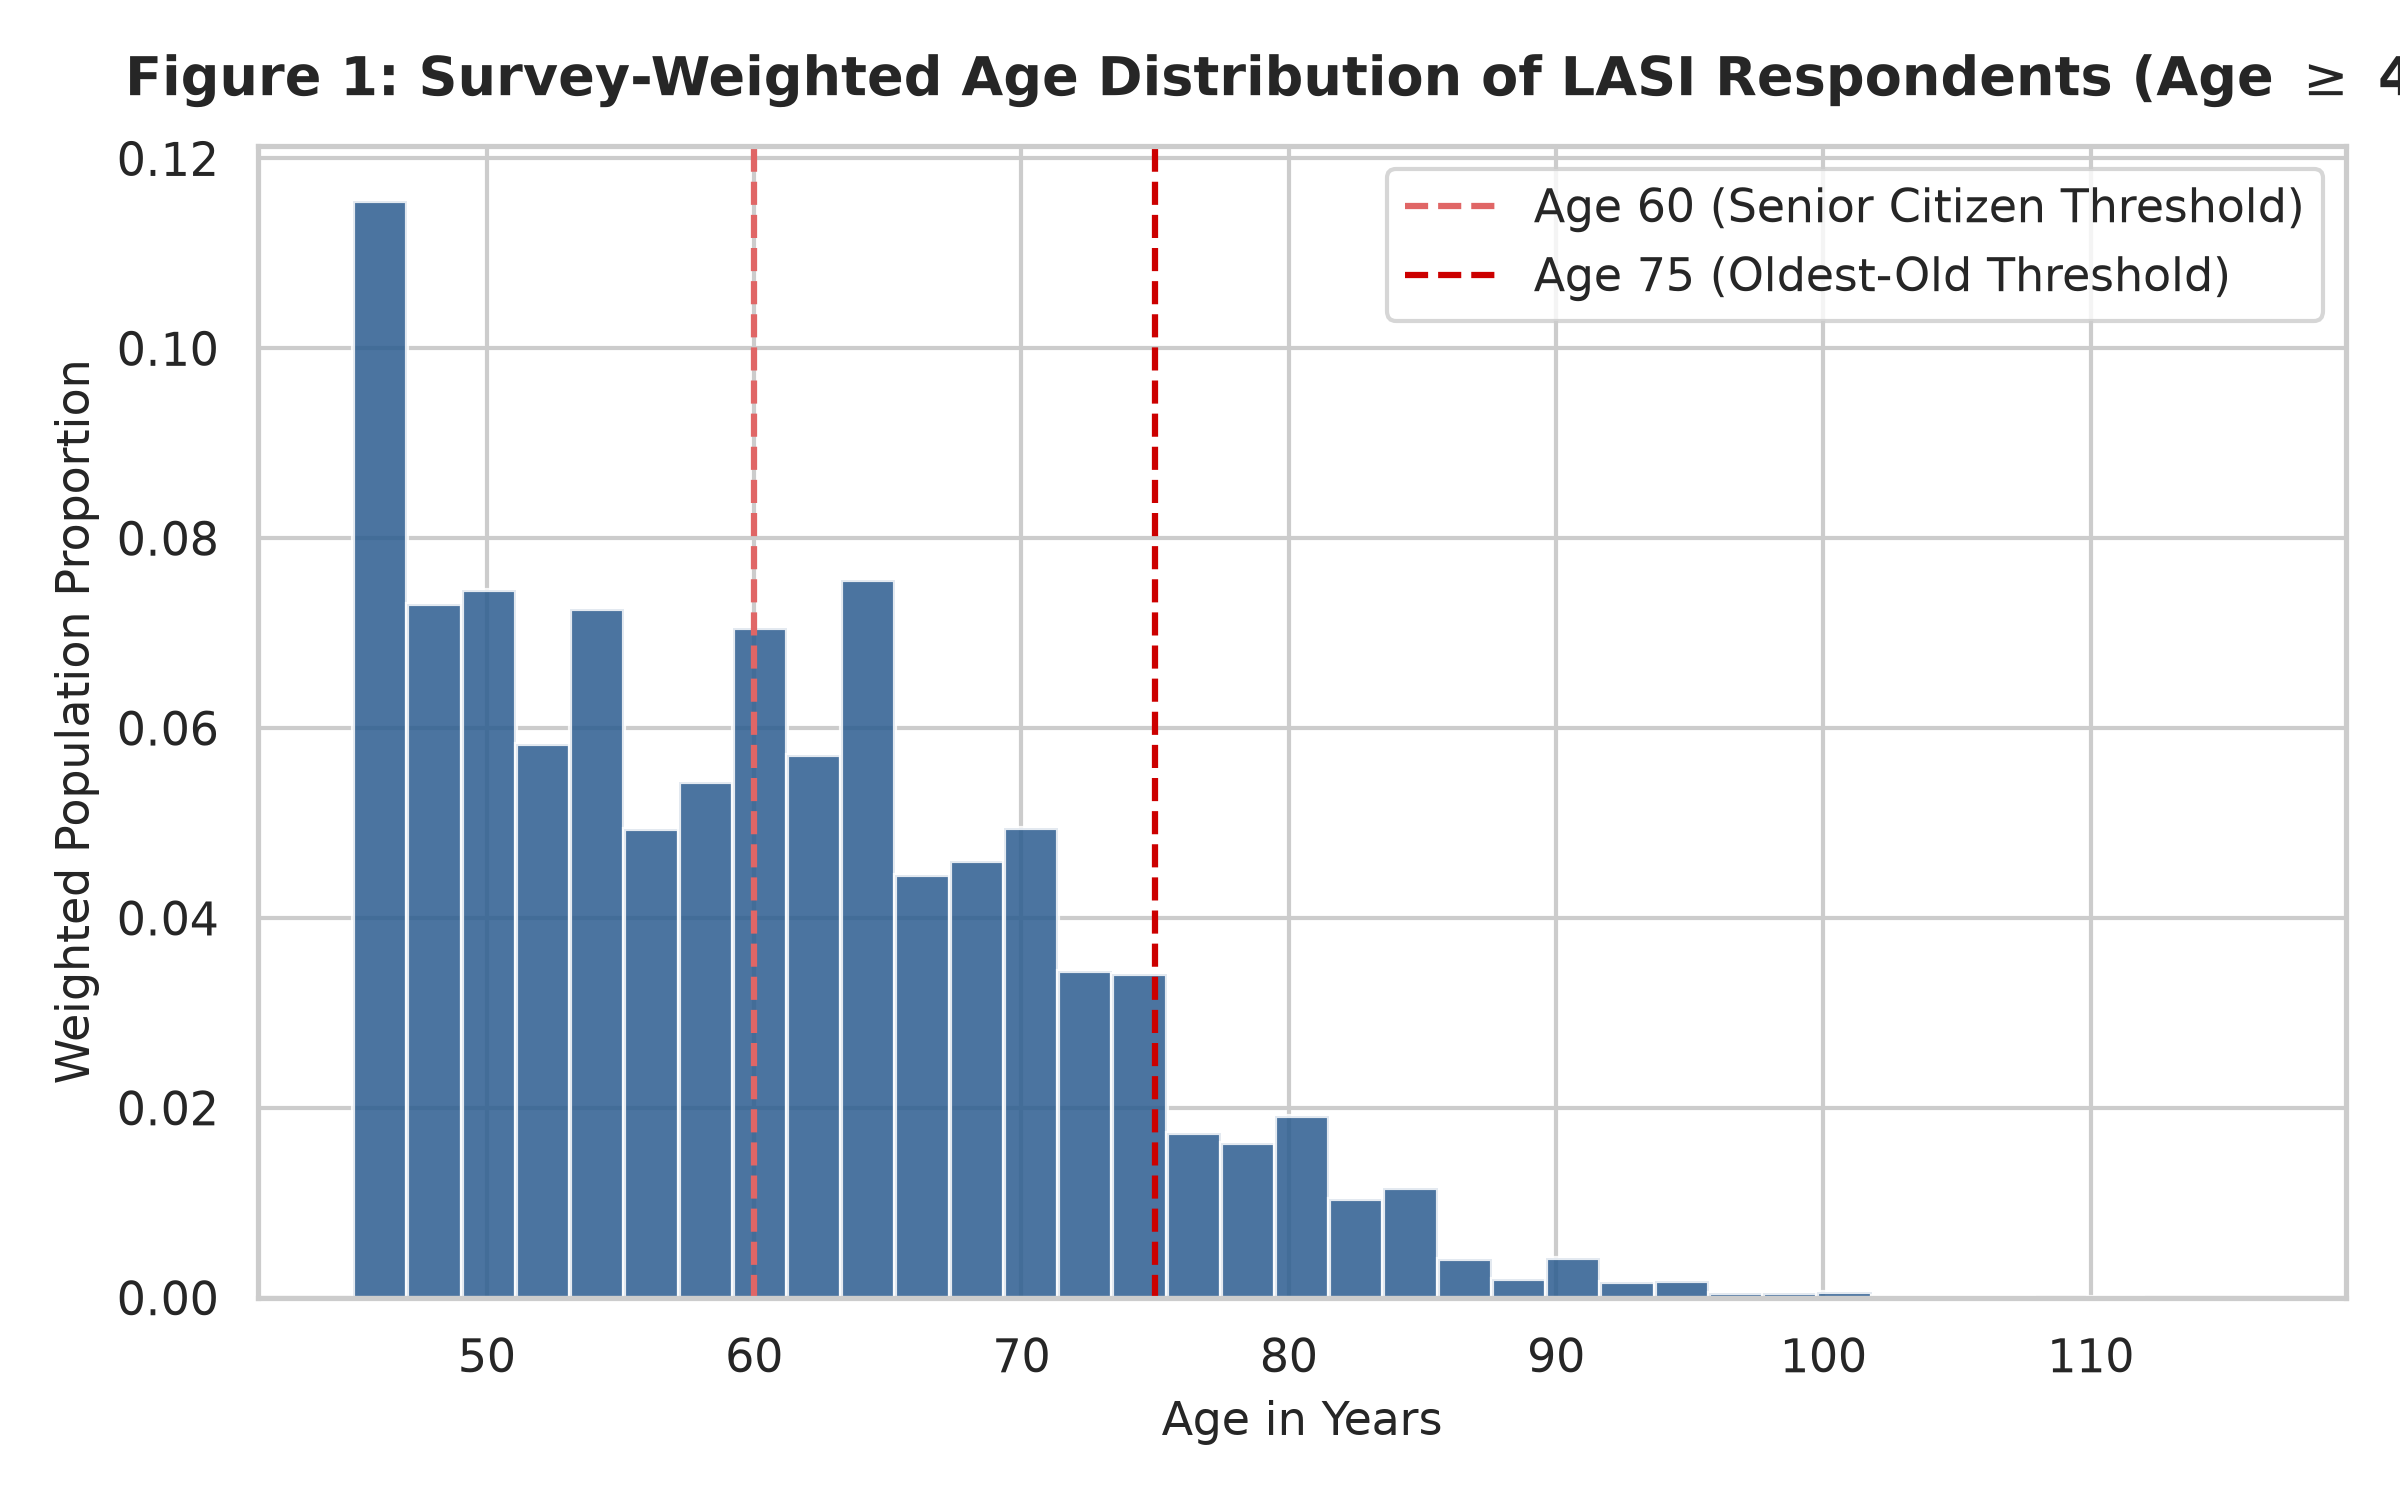
\includegraphics[width=0.75\textwidth]{figures/figure1_age_distribution.png}
    \caption{\textbf{Survey-Weighted Age Distribution of the Target Population ($\mathbf{N=66,606}$).} LASI Wave 1 adults aged 45 and older, displaying population proportions across five-year age bins and older-age milestones.}
    \label{fig:age_dist}
\end{figure}

\subsection{Exposure Definitions}
Childhood conditions (up to age 16) were measured via retrospective standardized interview modules:
\begin{enumerate}
    \item \textbf{Childhood Financial Status (\texttt{ht235}):} Self-rated financial status of the family during childhood: ``Pretty well-off financially'' (Reference, 7.8\% weighted), ``Average'' (49.3\%), ``Poor'' (42.2\%), and a voluntary category ``Varied'' (0.7\%, examined in sensitivity models).
    \item \textbf{Childhood Health Status (\texttt{ht231}):} General health status up to age 16: collapsed into ``Good'' (Very good [49.7\%] + Good [42.0\%], Reference) and ``Poor'' (Fair [7.1\%] + Poor [1.1\%] + Very poor [0.1\%]).
    \item \textbf{Childhood Bedridden Illness (\texttt{ht233}):} Binary indicator of whether the respondent was ever bedridden for a month or more due to a severe health condition before age 16 (Yes [5.4\%] vs. No [94.6\%]).
    \item \textbf{Cumulative Childhood Adversity Index:} An additive summary score (0 to 3) summing indicators for Poor childhood SES, Poor childhood health, and Bedridden illness.
\end{enumerate}

\begin{figure}[H]
    \centering
    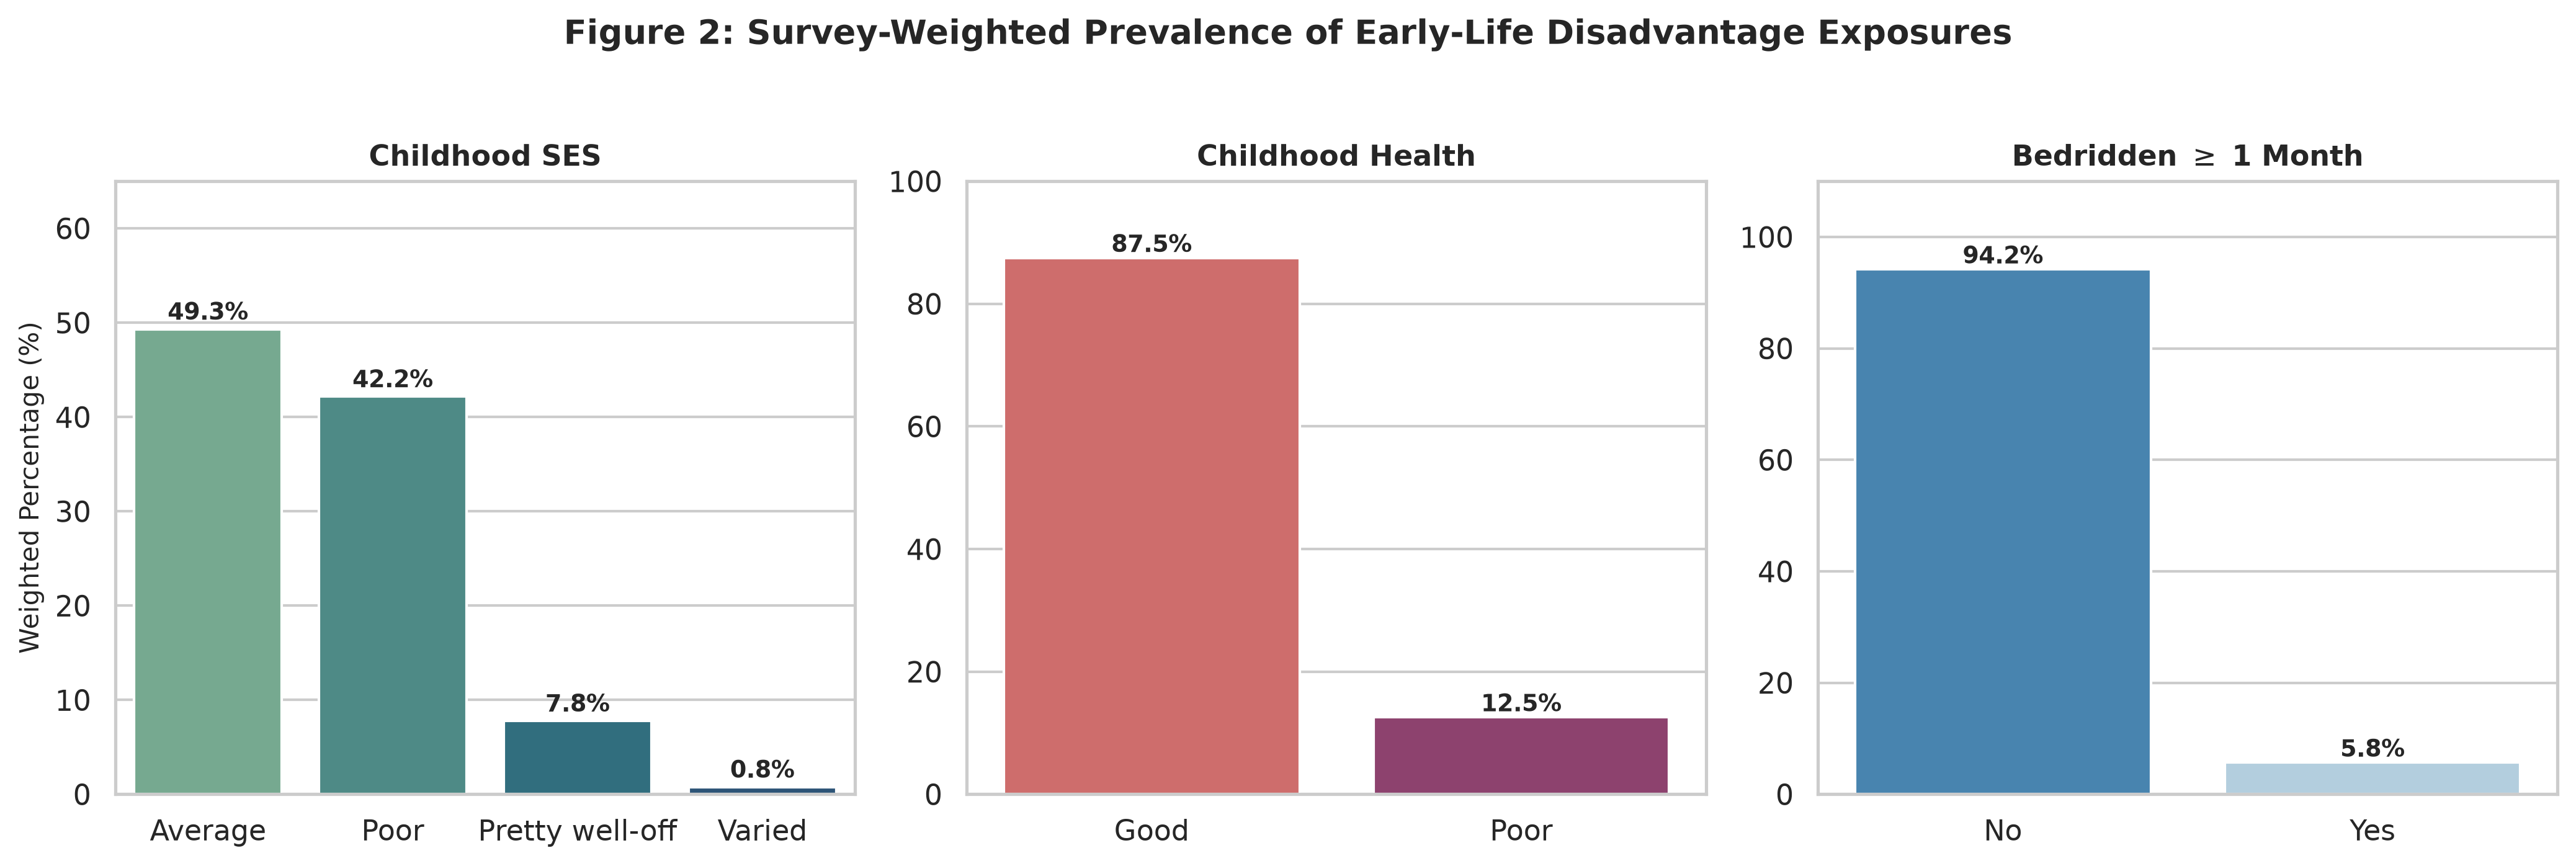
\includegraphics[width=0.75\textwidth]{figures/figure2_childhood_disadvantage_prevalence.png}
    \caption{\textbf{Survey-Weighted Prevalence of Early-Life Disadvantage Exposures.} Proportions of adults aged 45+ reporting adverse financial, general health, and serious bedridden conditions before age 16.}
    \label{fig:child_prev}
\end{figure}

\subsection{Outcome Definitions}

\subsubsection{Depressive Symptoms}
Depressive symptoms were assessed using the 10-item short form of the Center for Epidemiologic Studies Depression (CES-D) scale (\texttt{fs701}--\texttt{fs710}). The scale comprises seven negative affect items (trouble concentrating, feeling depressed, low energy, fearfulness, loneliness, being bothered, and feeling everything was an effort) and three positive affect items (overall satisfaction, hopefulness, and happiness). Items were scored binary (1 if symptom experienced often/most of the time during the past week; positive items reverse-coded). Respondents completing at least 8 items were included, with sum scores proportionally rescaled to 0--10 points. Clinical depressive symptoms were defined using the validated cutoff of $\text{CES-D} \ge 4.0$.

\subsubsection{Cognitive Performance and Impairment}
In LASI, direct cognitive assessments were administered exclusively to non-proxy respondents ($N = 65,901$). The protocol audit demonstrated that constructing an aggregate 43-point battery by replacing skipped literacy-dependent tasks (backward counting, serial 7 subtraction, paper folding, overlapping pentagon drawing) with zeros converted the cognitive score into a schooling artifact (Figure~\ref{fig:edu_grad}).

To resolve this confounder, the primary cognitive outcome was established as the \textbf{Memory and Orientation Composite (0--28 points)}:
\begin{itemize}
    \item Memory domain (0--20 points): Immediate 10-word recall (\texttt{mh012}) + Delayed 10-word recall (\texttt{mh056}).
    \item Orientation domain (0--8 points): Strict completion of all 8 temporal and spatial orientation items (date, month, year, day of week, place, village/town, district, landmark). Partial missingness was not scored as zero.
\end{itemize}
Binary \textbf{Cognitive Impairment} was established using the \textbf{survey-weighted 10th percentile cutoff} within the target population ($\le 11.0$ points), yielding a national weighted prevalence of 12.8\%.

For sensitivity, we evaluated:
\begin{itemize}
    \item \textit{Skip-Aware Full Battery (\% of maximum):} Domain proportions calculated strictly over items actually administered, preventing penalty for protocol-directed skips.
    \item \textit{Schooling-Stratum-Specific Deciles:} Impairment cutoffs calculated within educational strata (No formal education: $\le 10$; Low: $\le 12$; Middle: $\le 14$; High: $\le 16$).
    \item Continuous Memory+Orientation score (0--28) and continuous full battery.
\end{itemize}

\begin{figure}[H]
    \centering
    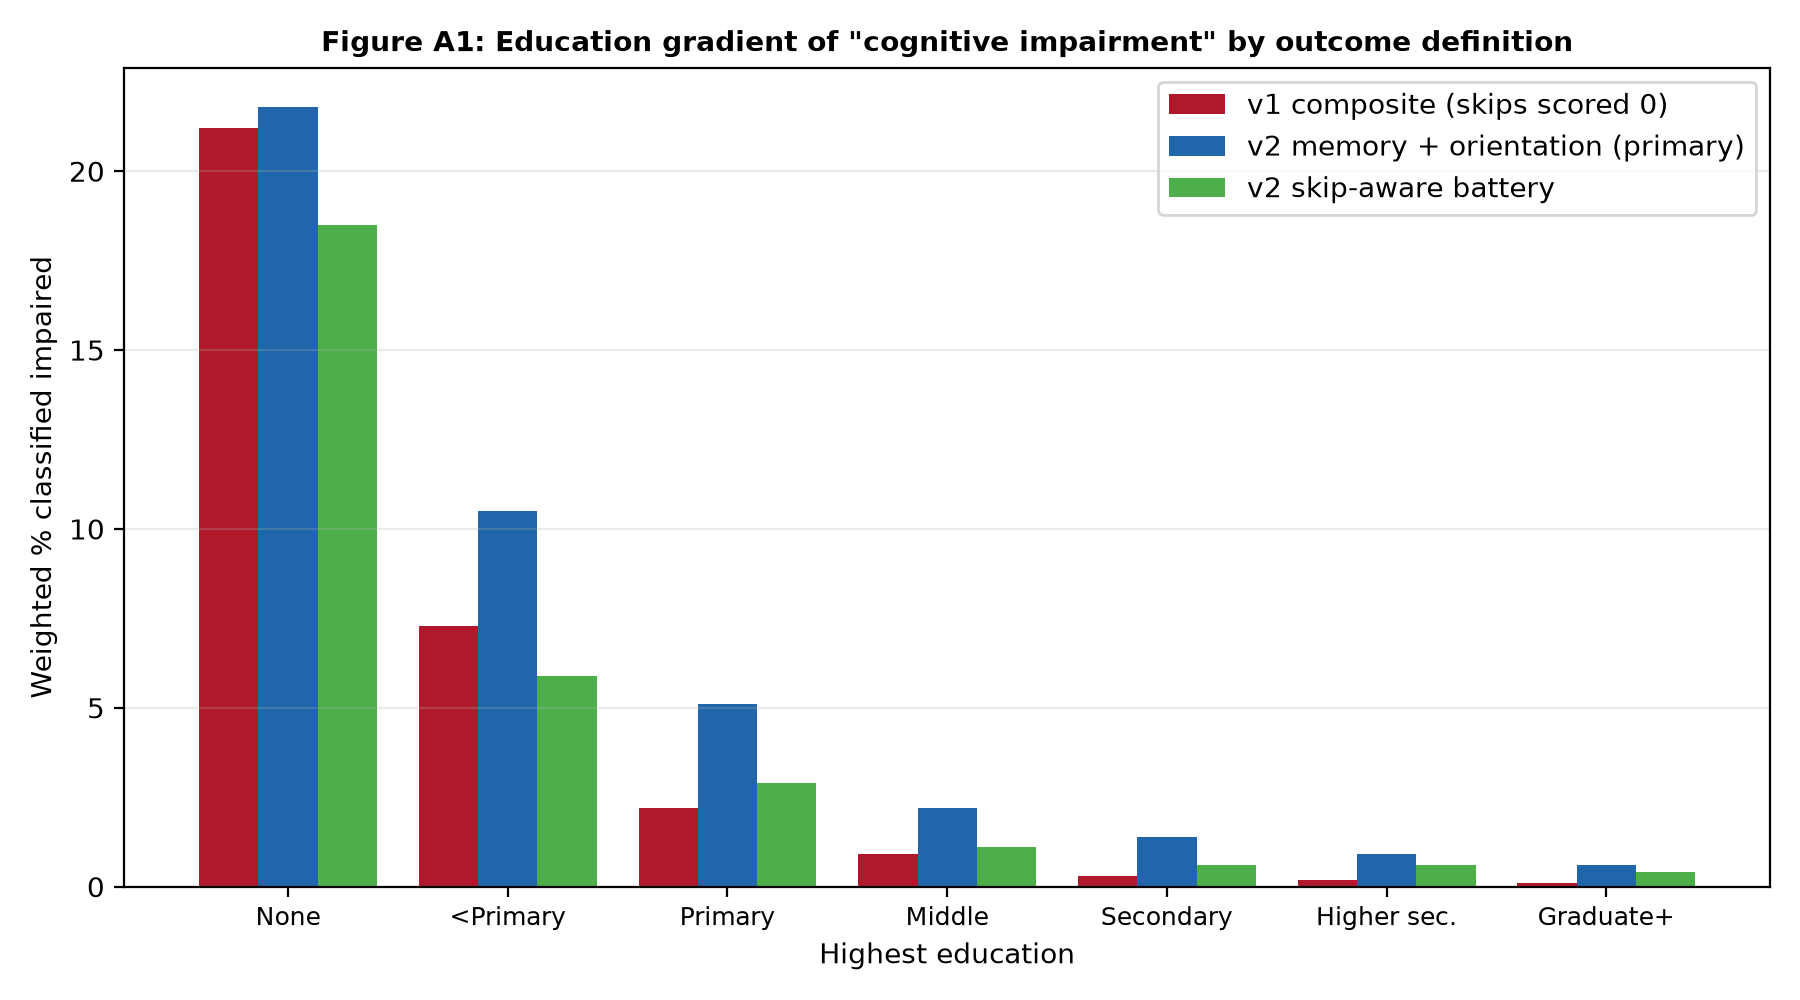
\includegraphics[width=0.75\textwidth]{figures/figureA1_education_gradient.png}
    \caption{\textbf{Classified Cognitive Impairment Gradient across Educational Strata.} Comparison between the unadjusted v1 composite (scoring skipped tasks as 0), the v2 memory and orientation primary outcome, and the skip-aware multi-domain battery.}
    \label{fig:edu_grad}
\end{figure}

\subsection{Statistical Estimation and Survey Weighting}

\subsubsection{Survey-Weighted Generalized Linear Models}
Because both depressive symptoms (28.2\%) and cognitive impairment (12.8\%) are common binary outcomes in this population, traditional logistic regression odds ratios (OR) substantially overestimate relative risk. We implemented survey-weighted \textbf{modified Poisson regression models} with a log-link function and robust variance estimators to compute adjusted \textbf{Prevalence Ratios (PR)} and 95\% Confidence Intervals:
\begin{equation}
    \log \left( \mathbb{E}[Y_i \mid \mathbf{X}_i] \right) = \beta_0 + \sum_{k} \beta_k X_{ik}
\end{equation}
Continuous outcomes (memory score, CES-D score) were modeled using survey-weighted Ordinary Least Squares (OLS).

\subsubsection{Stratified Cluster Variance Estimation}
Standard errors were calculated via Taylor series linearization accounting for the full multistage sampling design across 72 strata and 2,428 cluster PSUs. The sandwich covariance estimator was computed as:
\begin{equation}
    \mathbf{V} = \left( \mathbf{X}^T \mathbf{W} \mathbf{X} \right)^{-1} \mathbf{S} \left( \mathbf{X}^T \mathbf{W} \mathbf{X} \right)^{-1}
\end{equation}
where $\mathbf{S}$ denotes the between-cluster sum of score residuals centered within each stratum $h$:
\begin{equation}
    \mathbf{S} = \sum_{h=1}^{H} \frac{n_h}{n_h - 1} \sum_{c=1}^{n_h} \left( \mathbf{u}_{hc} - \bar{\mathbf{u}}_h \right) \left( \mathbf{u}_{hc} - \bar{\mathbf{u}}_h \right)^T
\end{equation}
Statistical inference was evaluated against the Student's $t$-distribution with degrees of freedom $df = \sum n_h - H = 2,428 - 72 = 2,356$.

\subsubsection{Model Hierarchy and Common Complete-Case Samples}
To prevent artificial changes in effect estimates caused by fluctuating sample sizes, all sequential models were fit on a single, invariant complete-case analytic sample:
\begin{itemize}
    \item \textbf{Cognition Sample:} $N = 57,245$ respondents (2,428 clusters, 72 strata).
    \item \textbf{Depression Sample:} $N = 62,047$ respondents (2,428 clusters, 72 strata).
\end{itemize}
The sequential covariate hierarchy was defined as:
\begin{itemize}
    \item \textbf{Model 0 (Unadjusted):} Outcome $\sim$ Childhood Exposure.
    \item \textbf{Model 1 (Demographic + Regional):} Model 0 + Continuous Age + Sex (Male vs. Female) + Residence (Rural vs. Urban) + Caste/Tribe (General/None, SC, ST, OBC, Other) + Marital Status (Married vs. Non-Married) + \textbf{36 State Fixed Effects}.
    \item \textbf{Model 2 (Adult SES -- Primary Model):} Model 1 + Educational Attainment (7 categories: No formal schooling, Less than primary, Primary, Middle, Secondary, Higher secondary/Diploma, Graduate and above) + Household Monthly Per Capita Consumption Expenditure (MPCE) Quintiles (1 Poorest to 5 Richest).
    \item \textbf{Model 3 (Adult Health Pathway -- Exploratory):} Model 2 + Chronic Morbidity Count (hypertension, diabetes, lung disease, heart disease, stroke: 0 to 5) + Concurrent Self-Rated Health (Excellent, Very good, Good, Fair, Poor).
\end{itemize}

\subsubsection{Effect Modification and Interaction Standardization}
Age heterogeneity was tested by including interaction terms between each exposure and age groups (45--59, 60--74, 75+) while retaining continuous age in the baseline specification. Rather than evaluating individual interaction coefficients, we computed \textbf{joint Wald $F$ tests} across all interaction degrees of freedom:
\begin{equation}
    F = \frac{\boldsymbol{\beta}_{\text{int}}^T \mathbf{V}_{\text{int}}^{-1} \boldsymbol{\beta}_{\text{int}}}{q}, \quad F \sim F(q, df - q + 1)
\end{equation}
To avoid unrepresentative single-profile predictions, we computed \textbf{Average Marginal Standardized Predictions (AME)} by evaluating model predictions across the observed empirical covariate distribution within each age stratum and calculating 95\% confidence intervals via 400 Monte Carlo draws from the parameter covariance matrix.

\subsubsection{Inverse-Probability Weighting (IPW) for Missing Cognition}
Because 7.8\% of cognitive tests were incomplete (rising to 19.9\% among adults aged 75+ and 13.3\% among unschooled individuals; Figure~\ref{fig:cog_miss}), we fit a multivariable logistic response model predicting complete cognitive assessment as a function of all exposures and Model 3 covariates. Weights were constructed as:
\begin{equation}
    w_i^{\text{IPW}} = w_i^{\text{survey}} \times \frac{1}{\widehat{P}(\text{Observed}_i \mid \mathbf{Z}_i)}
\end{equation}
Weights were trimmed at the 99th percentile and normalized to evaluate potential selection bias under the Missing at Random (MAR) assumption.

\begin{figure}[H]
    \centering
    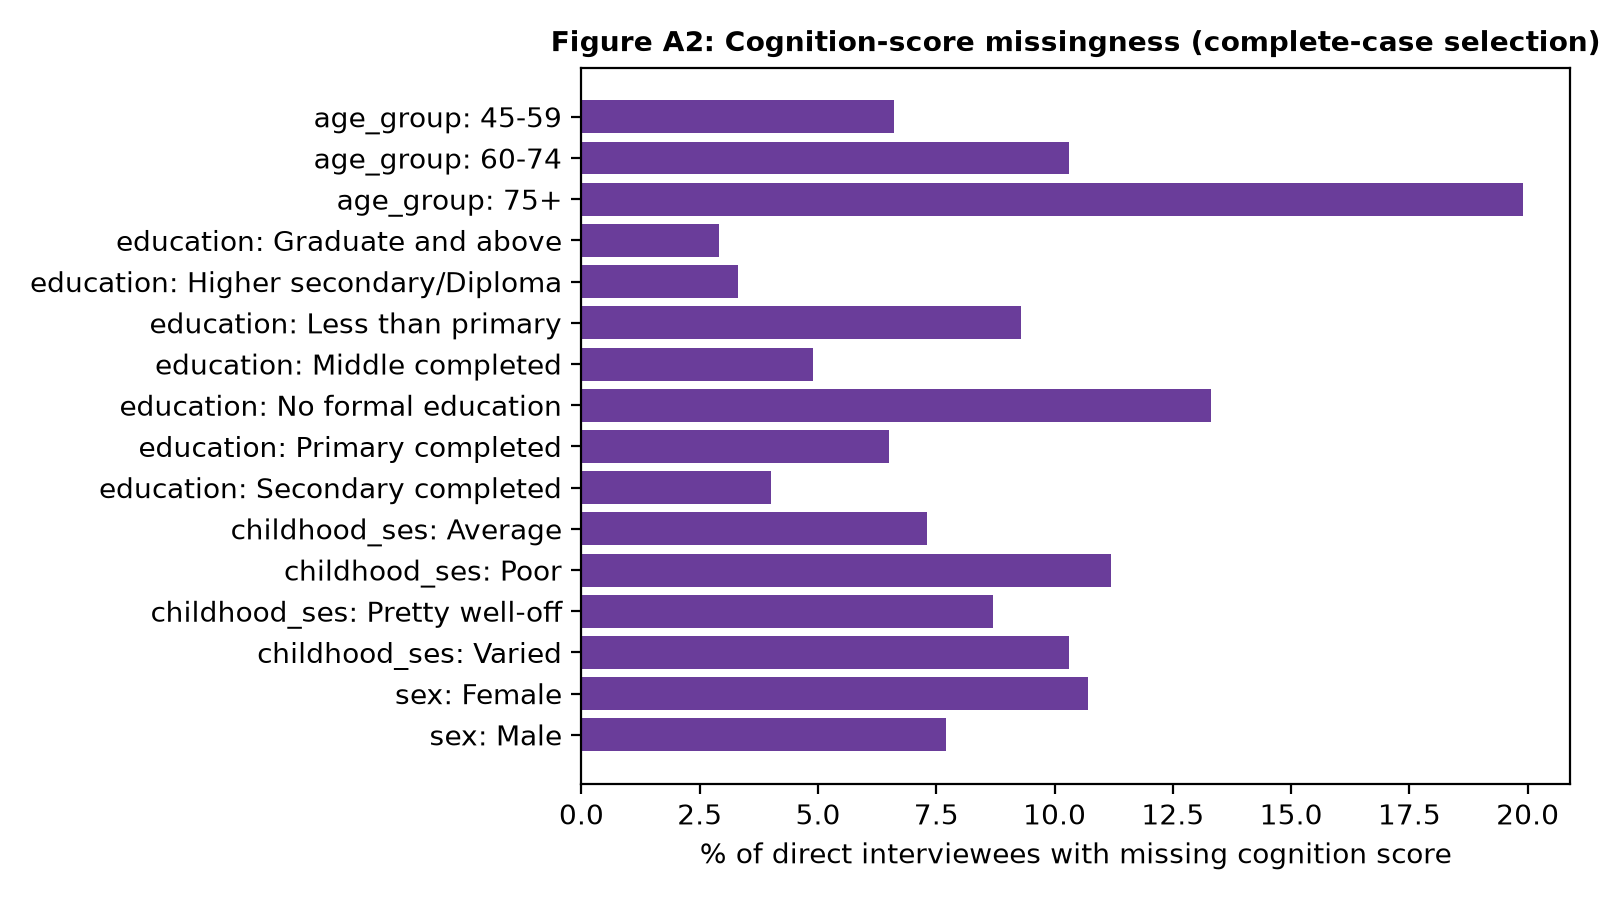
\includegraphics[width=0.75\textwidth]{figures/figureA2_cognition_missingness.png}
    \caption{\textbf{Proportion of Missing Cognitive Assessment Scores by Demographic and Socioeconomic Subgroups.} Missingness is heavily concentrated in the oldest-old (75+) and among unschooled adults, motivating IPW adjustments.}
    \label{fig:cog_miss}
\end{figure}

\section{Descriptive Results}

\subsection{Sample Characteristics}
Table~\ref{tab:sample_char} reports the survey-weighted demographic and socioeconomic distribution of the target population. Over 50\% of older Indian adults have no formal schooling, 68.5\% reside in rural sectors, and 42.2\% reported growing up in poor financial circumstances.

\begin{table}[H]
\centering
\small
\caption{\textbf{Baseline Sample Characteristics of Indian Adults Aged 45 and Older ($\mathbf{N=66,606}$).}}
\label{tab:sample_char}
\begin{tabular}{llrr}
\toprule
\textbf{Characteristic} & \textbf{Category} & \textbf{Unweighted N} & \textbf{Weighted \%} \\
\midrule
Age Group & 45-59 & 34,704 & 49.77\% \\
Age Group & 60-74 & 25,022 & 38.80\% \\
Age Group & 75+ & 6,880 & 11.42\% \\
Sex & Female & 35,567 & 54.06\% \\
Sex & Male & 31,039 & 45.94\% \\
Place of Residence & Rural & 43,240 & 68.53\% \\
Place of Residence & Urban & 23,366 & 31.47\% \\
Social Group / Caste & General/None & 16,295 & 24.84\% \\
Social Group / Caste & OBC & 25,212 & 46.66\% \\
Social Group / Caste & SC & 11,014 & 19.66\% \\
Social Group / Caste & ST & 11,746 & 8.84\% \\
Marital Status & Divorced/Separated & 1,006 & 1.23\% \\
Marital Status & Married/Partnered & 49,949 & 73.86\% \\
Marital Status & Never Married & 868 & 1.19\% \\
Marital Status & Widowed & 14,780 & 23.72\% \\
Educational Attainment & Graduate and above & 3,429 & 5.19\% \\
Educational Attainment & Higher secondary/Diploma & 3,175 & 4.94\% \\
Educational Attainment & Less than primary & 7,598 & 10.92\% \\
Educational Attainment & Middle completed & 6,337 & 8.35\% \\
Educational Attainment & No formal education & 31,350 & 50.62\% \\
Educational Attainment & Primary completed & 8,761 & 12.05\% \\
Educational Attainment & Secondary completed & 5,953 & 7.93\% \\
Household MPCE Quintile & 1 & 13,181 & 20.86\% \\
Household MPCE Quintile & 2 & 13,403 & 21.24\% \\
Household MPCE Quintile & 3 & 13,371 & 20.49\% \\
Household MPCE Quintile & 4 & 13,412 & 19.42\% \\
Household MPCE Quintile & 5 & 13,239 & 17.99\% \\
Childhood SES & Average & 35,438 & 49.32\% \\
Childhood SES & Poor & 25,605 & 42.16\% \\
Childhood SES & Pretty well-off & 4,848 & 7.77\% \\
Childhood SES & Varied & 394 & 0.76\% \\
Childhood Health & Good & 58,272 & 87.46\% \\
Childhood Health & Poor & 7,369 & 12.54\% \\
Childhood Bedridden & No & 62,881 & 94.25\% \\
Childhood Bedridden & Yes & 3,370 & 5.75\% \\
Cumulative Disadvantage Score & 0.0 & 34,506 & 48.19\% \\
Cumulative Disadvantage Score & 1.0 & 26,556 & 44.06\% \\
Cumulative Disadvantage Score & 2.0 & 4,003 & 6.86\% \\
Cumulative Disadvantage Score & 3.0 & 466 & 0.88\% \\
\bottomrule
\end{tabular}
\end{table}

\subsection{Outcome Prevalence Across Age Strata}
Table~\ref{tab:outcomes_age} presents survey-weighted prevalence and domain mean scores across age groups with design-based 95\% confidence intervals. The prevalence of cognitive impairment rises steeply from 7.61\% in mid-life (45--59) to 28.85\% among the oldest-old (75+). Depressive symptoms similarly show an upward gradient from 26.28\% to 34.18\%.

\begin{table}[H]
\centering
\small
\caption{\textbf{Weighted Prevalence and Means of Health Outcomes across Age Strata (Design-Based 95\% CIs).}}
\label{tab:outcomes_age}
\begin{tabular}{llrrr}
\toprule
\textbf{Age Group} & \textbf{Outcome Measure} & \textbf{Estimate} & \textbf{95\% Confidence Interval} & \textbf{Sample N} \\
\midrule
45-59 & Cognitive impairment (\%) & 7.61 & (7.00--8.22) & 32,301 \\
45-59 & Depressive symptoms (\%) & 26.28 & (24.99--27.58) & 34,009 \\
45-59 & Mem+orient score (mean, 0-28) & 17.01 & (16.85--17.17) & 32,301 \\
45-59 & CES-D score (mean) & 2.86 & (2.81--2.91) & 34,009 \\
60-74 & Cognitive impairment (\%) & 15.61 & (14.58--16.65) & 22,223 \\
60-74 & Depressive symptoms (\%) & 29.10 & (27.80--30.41) & 24,370 \\
60-74 & Mem+orient score (mean, 0-28) & 15.51 & (15.38--15.65) & 22,223 \\
60-74 & CES-D score (mean) & 3.01 & (2.95--3.06) & 24,370 \\
75+ & Cognitive impairment (\%) & 28.85 & (26.20--31.50) & 5,257 \\
75+ & Depressive symptoms (\%) & 34.18 & (31.02--37.33) & 6,446 \\
75+ & Mem+orient score (mean, 0-28) & 13.88 & (13.65--14.11) & 5,257 \\
75+ & CES-D score (mean) & 3.27 & (3.15--3.39) & 6,446 \\
All & Cognitive impairment (\%) & 12.79 & (12.03--13.54) & 59,781 \\
All & Depressive symptoms (\%) & 28.24 & (27.19--29.28) & 64,825 \\
All & Mem+orient score (mean, 0-28) & 16.13 & (16.00--16.25) & 59,781 \\
All & CES-D score (mean) & 2.96 & (2.92--3.00) & 64,825 \\
\bottomrule
\end{tabular}
\end{table}

\section{Primary Regression Findings}

\subsection{Cognitive Impairment: Attenuation by Adult Socioeconomic Attainment}
Table~\ref{tab:cog_reg} presents sequential modified Poisson models for cognitive impairment. In unadjusted models (Model 0), adults from poor childhood backgrounds had a 61\% higher prevalence of cognitive impairment ($\text{PR} = 1.61$, 95\% CI: 1.33--1.96, $p < 0.001$). Adjusting for demographics and state fixed effects (Model 1) attenuated this to 36\% ($\text{PR} = 1.36$, 95\% CI: 1.16--1.59, $p < 0.001$).

Crucially, upon adjusting for adult educational attainment and household consumption expenditure (Model 2), the association was \textbf{completely eliminated} ($\text{APR} = 0.93$, 95\% CI: 0.82--1.05, $p = 0.241$). Childhood health and bedridden illness demonstrated no significant associations with cognitive impairment across any model specifications ($\text{APR} \approx 0.95$--$1.00$).

On the continuous memory and orientation score (Table~\ref{tab:cog_cont}), poor childhood SES was associated with a modest adjusted deficit of $-0.32$ points (95\% CI: $-0.56$ to $-0.09$, $p = 0.008$), representing a 75\% attenuation from the demographic-adjusted estimate ($-1.28$ points).

\begin{table}[H]
\centering
\small
\caption{\textbf{Sequential Survey-Weighted Modified Poisson Regressions for Cognitive Impairment ($\mathbf{N=57,245}$).}}
\label{tab:cog_reg}
\resizebox{\textwidth}{!}{%
\begin{tabular}{lcccc}
\toprule
\textbf{Childhood Exposure Parameter} & \textbf{Model 0: Unadj.} & \textbf{Model 1: Demog.+State} & \textbf{Model 2: +Adult SES (Primary)} & \textbf{Model 3: +Adult Health} \\
\midrule
Childhood SES: Average & 0.97 (0.82--1.15) \textit{p}=0.711 & 0.98 (0.84--1.14) \textit{p}=0.777 & 0.80 (0.70--0.91) \textit{p}$<$0.001 & 0.80 (0.71--0.91) \textit{p}$<$0.001 \\
Childhood SES: Poor & 1.61 (1.33--1.96) \textit{p}$<$0.001 & 1.36 (1.16--1.59) \textit{p}$<$0.001 & 0.93 (0.82--1.05) \textit{p}=0.241 & 0.91 (0.81--1.03) \textit{p}=0.148 \\
Childhood bedridden $\ge$1 month & 0.90 (0.77--1.06) \textit{p}=0.222 & 0.94 (0.81--1.09) \textit{p}=0.404 & 1.00 (0.86--1.18) \textit{p}=0.947 & 0.99 (0.84--1.16) \textit{p}=0.868 \\
Childhood health: Fair/Poor/Very poor & 0.97 (0.81--1.17) \textit{p}=0.773 & 0.97 (0.85--1.12) \textit{p}=0.719 & 0.95 (0.82--1.10) \textit{p}=0.487 & 0.95 (0.82--1.09) \textit{p}=0.458 \\
\bottomrule
\end{tabular}%
}
\end{table}

\begin{table}[H]
\centering
\small
\caption{\textbf{Continuous Memory and Orientation Score Regressions (Linear Survey OLS, Beta Coefficients, $\mathbf{N=57,245}$).}}
\label{tab:cog_cont}
\resizebox{\textwidth}{!}{%
\begin{tabular}{lcccc}
\toprule
\textbf{Exposure (vs. Reference)} & \textbf{Model 0: Unadjusted} & \textbf{Model 1: Demog.+State} & \textbf{Model 2: +Adult SES} & \textbf{Model 3: +Adult Health} \\
\midrule
Childhood SES: Poor & $-1.65$ ($-1.95$--$-1.34$) & $-1.28$ ($-1.54$--$-1.02$) & $-0.32$ ($-0.56$--$-0.09$) & $-0.25$ ($-0.48$--$-0.01$) \\
Childhood Health: Poor & $-0.02$ ($-0.43$--$0.39$) & $-0.05$ ($-0.29$--$0.18$) & $+0.01$ ($-0.23$--$0.25$) & $+0.04$ ($-0.19$--$0.27$) \\
Childhood Bedridden: Yes & $+0.14$ ($-0.25$--$0.53$) & $+0.02$ ($-0.19$--$0.23$) & $-0.15$ ($-0.35$--$0.05$) & $-0.10$ ($-0.30$--$0.10$) \\
\bottomrule
\end{tabular}%
}
\end{table}

\subsection{Depressive Symptoms: Enduring Somatic and Socioeconomic Scarring}
In sharp contrast to cognitive outcomes, Table~\ref{tab:dep_reg} demonstrates that early-life disadvantage exerts \textbf{enduring, non-attenuated associations with later-life depressive symptoms}. In primary Model 2, depressive symptoms were significantly elevated among individuals who experienced poor childhood health ($\text{APR} = 1.20$, 95\% CI: 1.07--1.34, $p = 0.002$), poor childhood SES ($\text{APR} = 1.21$, 95\% CI: 1.03--1.42, $p = 0.019$), and childhood bedridden illness ($\text{APR} = 1.16$, 95\% CI: 1.05--1.28, $p = 0.005$).

Even after further conditioning on adult chronic multimorbidity and concurrent self-rated health in Model 3, childhood health ($\text{APR} = 1.19$, 95\% CI: 1.06--1.33) and bedridden illness ($\text{APR} = 1.11$, 95\% CI: 1.01--1.23) remained independently associated with depressive symptoms.

\begin{table}[H]
\centering
\small
\caption{\textbf{Sequential Survey-Weighted Modified Poisson Regressions for Depressive Symptoms ($\mathbf{N=62,047}$).}}
\label{tab:dep_reg}
\resizebox{\textwidth}{!}{%
\begin{tabular}{lcccc}
\toprule
\textbf{Childhood Exposure Parameter} & \textbf{Model 0: Unadj.} & \textbf{Model 1: Demog.+State} & \textbf{Model 2: +Adult SES (Primary)} & \textbf{Model 3: +Adult Health} \\
\midrule
Childhood SES: Average & 1.10 (0.94--1.30) \textit{p}=0.233 & 1.20 (1.01--1.44) \textit{p}=0.039 & 1.15 (0.99--1.33) \textit{p}=0.072 & 1.14 (0.99--1.32) \textit{p}=0.071 \\
Childhood SES: Poor & 1.17 (1.00--1.37) \textit{p}=0.044 & 1.31 (1.09--1.58) \textit{p}=0.004 & 1.21 (1.03--1.42) \textit{p}=0.019 & 1.15 (0.99--1.34) \textit{p}=0.068 \\
Childhood bedridden $\ge$1 month & 1.14 (1.01--1.29) \textit{p}=0.037 & 1.14 (1.01--1.27) \textit{p}=0.034 & 1.16 (1.05--1.28) \textit{p}=0.004 & 1.11 (1.01--1.23) \textit{p}=0.029 \\
Childhood health: Fair/Poor/Very poor & 1.33 (1.20--1.47) \textit{p}$<$0.001 & 1.21 (1.08--1.36) \textit{p}=0.002 & 1.20 (1.07--1.34) \textit{p}=0.002 & 1.19 (1.06--1.33) \textit{p}=0.002 \\
\bottomrule
\end{tabular}%
}
\end{table}

\begin{figure}[H]
    \centering
    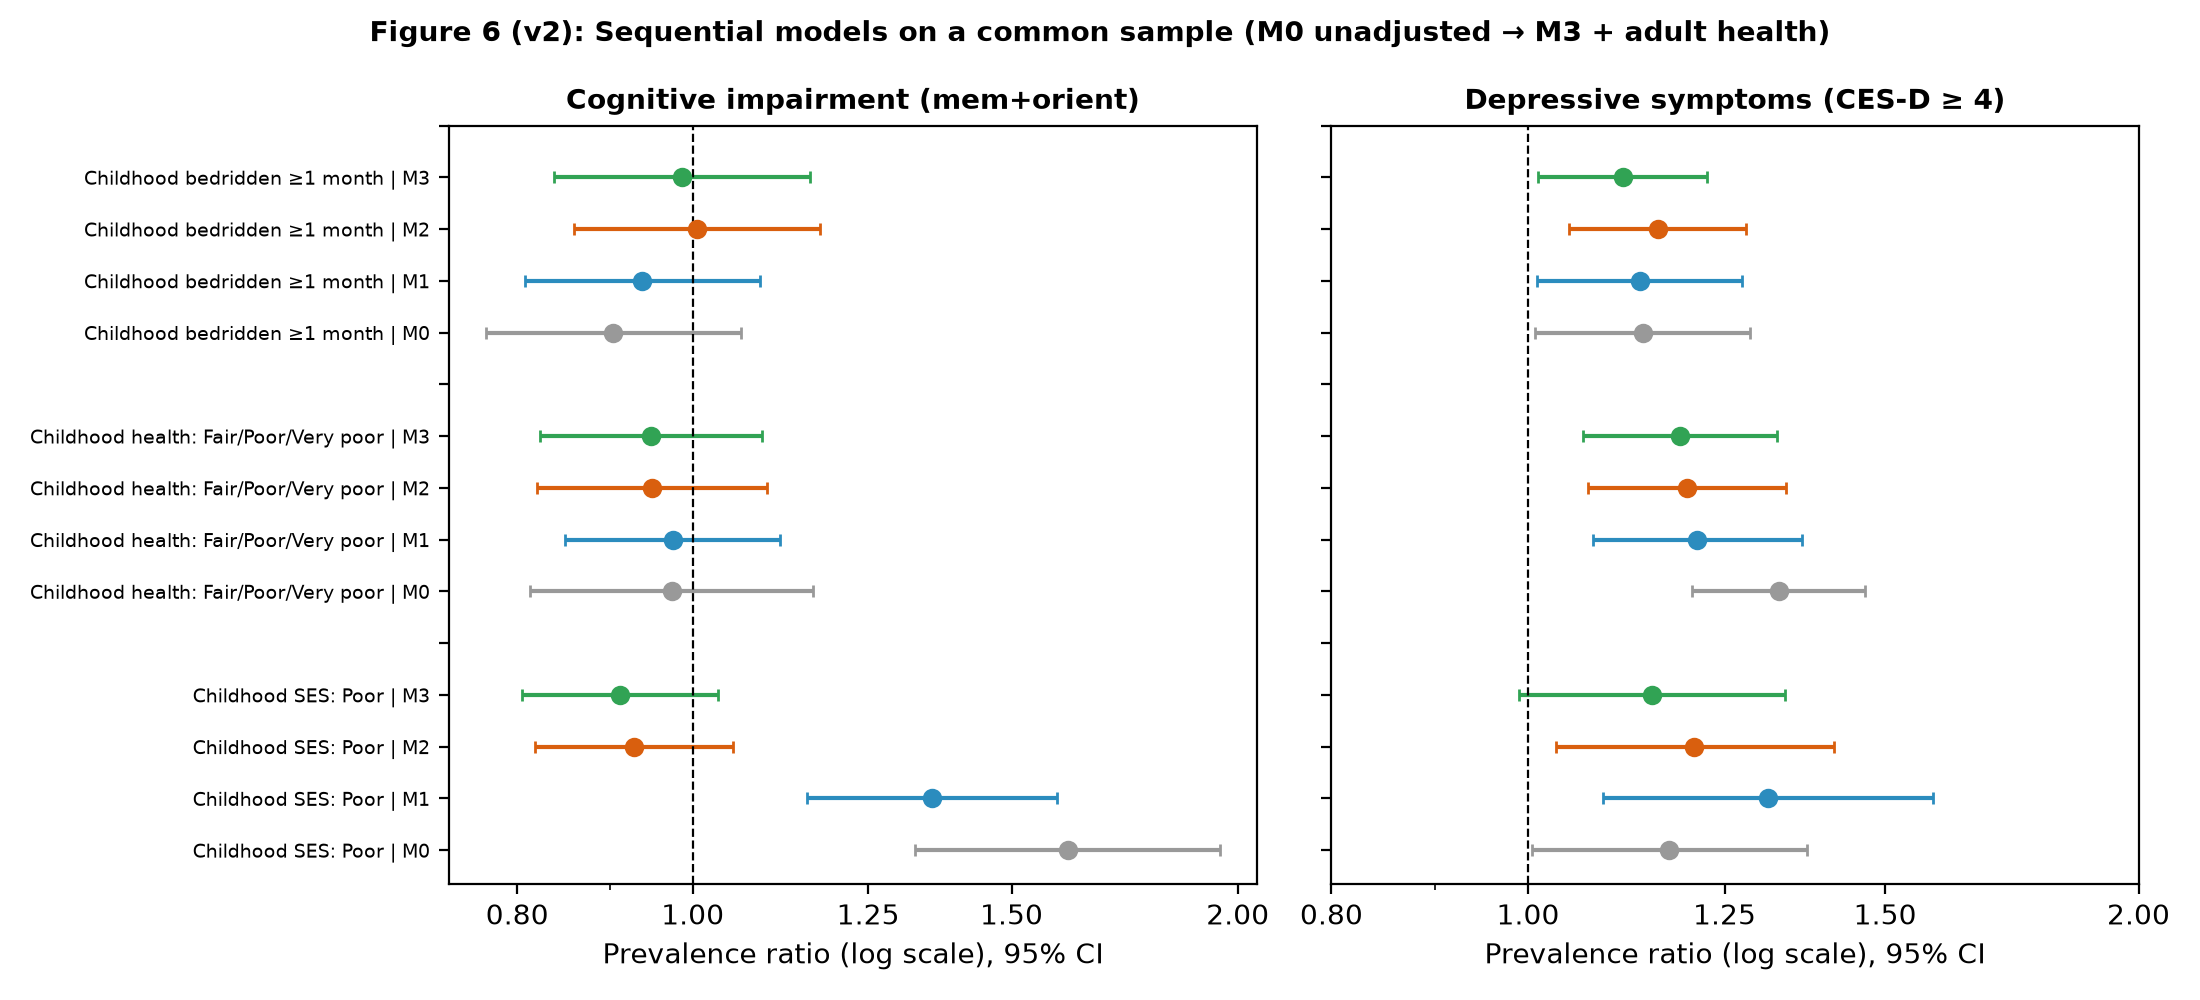
\includegraphics[width=0.92\textwidth]{figures/figure6v2_forest_sequential.png}
    \caption{\textbf{Sequential Model Forest Plots for Cognitive Impairment and Depressive Symptoms.} Contrasting the attenuation of cognitive disparities after adult SES adjustment against the enduring persistence of depressive symptom disparities.}
    \label{fig:forest}
\end{figure}

\subsection{Mutually Adjusted Models and Cumulative Disadvantage}
When all childhood exposures were included simultaneously in the same regression equation (Table~\ref{tab:mutual}), childhood SES ($\text{APR} = 1.19$, 95\% CI: 1.02--1.38), poor childhood health ($\text{APR} = 1.18$, 95\% CI: 1.05--1.32), and childhood bedridden illness ($\text{APR} = 1.12$, 95\% CI: 1.00--1.26) maintained independent, non-overlapping associations with later-life depression.

Evaluating the \textbf{Cumulative Disadvantage Index} demonstrated a clear linear dose-response relationship: each additional childhood adversity increased the adjusted prevalence of depressive symptoms by \textbf{11.4\%} ($\text{APR} = 1.114$, 95\% CI: 1.070--1.160, $p < 0.001$). For cognitive impairment, the cumulative index was not statistically significant after adult SES controls ($\text{APR} = 1.054$, 95\% CI: 0.995--1.117, $p = 0.071$).

\begin{table}[H]
\centering
\small
\caption{\textbf{Mutually Adjusted Childhood Models and Cumulative Disadvantage Score.}}
\label{tab:mutual}
\resizebox{\textwidth}{!}{%
\begin{tabular}{llcc}
\toprule
\textbf{Model Hierarchy} & \textbf{Childhood Exposure Parameter} & \textbf{Prevalence Ratio (95\% CI)} & \textbf{\textit{p}-value} \\
\midrule
\multicolumn{4}{l}{\textbf{Panel A: Cognitive Impairment ($N = 57,245$)}} \\
\midrule
Model 1: Demographics + state & Childhood SES: Average & 0.98 (0.84--1.14) & $0.792$ \\
Model 1: Demographics + state & Childhood SES: Poor & 1.36 (1.15--1.60) & $<0.001$ \\
Model 1: Demographics + state & Childhood health: Fair/Poor/Very poor & 0.97 (0.84--1.12) & $0.681$ \\
Model 1: Demographics + state & Childhood bedridden $\ge$1 month & 0.94 (0.81--1.10) & $0.430$ \\
Model 2: + Adult SES (Primary) & Childhood SES: Average & 0.80 (0.70--0.91) & $<0.001$ \\
Model 2: + Adult SES (Primary) & Childhood SES: Poor & 0.93 (0.82--1.06) & $0.277$ \\
Model 2: + Adult SES (Primary) & Childhood health: Fair/Poor/Very poor & 0.95 (0.82--1.10) & $0.533$ \\
Model 2: + Adult SES (Primary) & Childhood bedridden $\ge$1 month & 1.01 (0.86--1.18) & $0.941$ \\
Model 3: + Adult health (Pathway) & Childhood SES: Average & 0.81 (0.71--0.92) & $0.001$ \\
Model 3: + Adult health (Pathway) & Childhood SES: Poor & 0.91 (0.81--1.04) & $0.171$ \\
Model 3: + Adult health (Pathway) & Childhood health: Fair/Poor/Very poor & 0.95 (0.83--1.10) & $0.514$ \\
Model 3: + Adult health (Pathway) & Childhood bedridden $\ge$1 month & 0.99 (0.84--1.17) & $0.892$ \\
Model 2: + Adult SES (Primary) (Cumulative) & Per additional childhood adversity & 1.05 (0.99--1.12) & $0.071$ \\
\midrule
\multicolumn{4}{l}{\textbf{Panel B: Depressive Symptoms ($N = 62,047$)}} \\
\midrule
Model 1: Demographics + state & Childhood SES: Average & 1.18 (1.00--1.39) & $0.044$ \\
Model 1: Demographics + state & Childhood SES: Poor & 1.29 (1.08--1.54) & $0.005$ \\
Model 1: Demographics + state & Childhood health: Fair/Poor/Very poor & 1.19 (1.05--1.34) & $0.005$ \\
Model 1: Demographics + state & Childhood bedridden $\ge$1 month & 1.10 (0.97--1.25) & $0.147$ \\
Model 2: + Adult SES (Primary) & Childhood SES: Average & 1.13 (0.98--1.29) & $0.090$ \\
Model 2: + Adult SES (Primary) & Childhood SES: Poor & 1.19 (1.02--1.38) & $0.026$ \\
Model 2: + Adult SES (Primary) & Childhood health: Fair/Poor/Very poor & 1.18 (1.05--1.32) & $0.006$ \\
Model 2: + Adult SES (Primary) & Childhood bedridden $\ge$1 month & 1.12 (1.00--1.26) & $0.044$ \\
Model 3: + Adult health (Pathway) & Childhood SES: Average & 1.12 (0.98--1.29) & $0.087$ \\
Model 3: + Adult health (Pathway) & Childhood SES: Poor & 1.13 (0.98--1.31) & $0.089$ \\
Model 3: + Adult health (Pathway) & Childhood health: Fair/Poor/Very poor & 1.17 (1.05--1.31) & $0.006$ \\
Model 3: + Adult health (Pathway) & Childhood bedridden $\ge$1 month & 1.08 (0.97--1.21) & $0.157$ \\
Model 2: + Adult SES (Primary) (Cumulative) & Per additional childhood adversity & 1.11 (1.07--1.16) & $<0.001$ \\
\bottomrule
\end{tabular}%
}
\end{table}

\section{Age Heterogeneity and Interaction Analysis}

\subsection{Formal Tests of Effect Modification (Hypothesis 4)}
To test Hypothesis 4 (that early disadvantage compounds across ageing stages or diminishes due to mortality selection), we conducted joint Wald $F$ tests across all exposure-by-age interactions (Table~\ref{tab:joint_test}).

For depressive symptoms, all joint interaction tests were firmly null: Childhood SES $\times$ Age ($F = 0.34, p = 0.851$), Childhood Health $\times$ Age ($F = 0.31, p = 0.736$), and Bedridden $\times$ Age ($F = 0.02, p = 0.980$). The association between childhood adversity and late-life depression is remarkably uniform across middle and older adulthood.

For cognitive impairment, the joint interaction between Childhood SES and Age reached marginal significance ($F = 2.44, p = 0.045$). However, this nominal effect was driven entirely by an anomalous inversion in the oldest-old stratum (75+), where adults from ``Pretty well-off'' childhoods had a higher standardized predicted prevalence of cognitive impairment (36.9\%, 95\% CI: 30.9--44.0) than those from poor childhoods (28.0\%, 95\% CI: 26.1--31.4; Table~\ref{tab:risk_diff}). Because this nominal interaction is in the opposite direction of theoretical expectations and does not survive multiple testing correction ($\alpha / 6 = 0.008$), \textbf{Hypothesis 4 is not supported}.

\begin{table}[H]
\centering
\small
\caption{\textbf{Joint Wald $\mathbf{F}$ Tests for Age-Group Interactions ($\mathbf{\text{Exposure} \times \text{Age Group}}$).}}
\label{tab:joint_test}
\resizebox{\textwidth}{!}{%
\begin{tabular}{llcccc}
\toprule
\textbf{Health Outcome} & \textbf{Tested Childhood Exposure} & \textbf{Joint Wald \textit{F}} & \textbf{Numerator \textit{df}} & \textbf{\textit{p}-value} & \textbf{Sample N} \\
\midrule
Cognitive impairment & Childhood SES & 2.439 & 4 & $0.045$ & 57,245 \\
Cognitive impairment & Childhood health & 0.322 & 2 & $0.725$ & 57,245 \\
Cognitive impairment & Childhood bedridden & 0.271 & 2 & $0.763$ & 57,245 \\
Depressive symptoms & Childhood SES & 0.340 & 4 & $0.851$ & 62,047 \\
Depressive symptoms & Childhood health & 0.306 & 2 & $0.736$ & 62,047 \\
Depressive symptoms & Childhood bedridden & 0.021 & 2 & $0.980$ & 62,047 \\
\bottomrule
\end{tabular}%
}
\end{table}

\begin{table}[H]
\centering
\small
\caption{\textbf{Average Marginal Standardized Risk Differences across Age Groups.}}
\label{tab:risk_diff}
\resizebox{\textwidth}{!}{%
\begin{tabular}{lllc}
\toprule
\textbf{Childhood Exposure} & \textbf{Age Group} & \textbf{Tested Contrast} & \textbf{Risk Difference, pp (95\% CI)} \\
\midrule
\multicolumn{4}{l}{\textbf{Panel A: Cognitive Impairment ($N = 57,245$)}} \\
\midrule
Childhood SES & 45-59 & Poor - Pretty well-off & +0.29 (-1.91 to +1.95) \\
Childhood SES & 60-74 & Poor - Pretty well-off & -0.71 (-3.94 to +2.07) \\
Childhood SES & 75+ & Poor - Pretty well-off & -8.83 (-16.21 to -1.38) \\
Childhood health & 45-59 & Poor - Good & -0.72 (-2.39 to +1.02) \\
Childhood health & 60-74 & Poor - Good & -0.12 (-2.54 to +2.64) \\
Childhood health & 75+ & Poor - Good & -2.42 (-8.63 to +4.82) \\
Childhood bedridden & 45-59 & Yes - No & +0.56 (-0.90 to +2.26) \\
Childhood bedridden & 60-74 & Yes - No & -0.62 (-3.65 to +2.95) \\
Childhood bedridden & 75+ & Yes - No & -0.04 (-10.44 to +16.22) \\
\midrule
\multicolumn{4}{l}{\textbf{Panel B: Depressive Symptoms ($N = 62,047$)}} \\
\midrule
Childhood SES & 45-59 & Poor - Pretty well-off & +4.32 (+0.57 to +7.77) \\
Childhood SES & 60-74 & Poor - Pretty well-off & +6.20 (+0.92 to +10.95) \\
Childhood SES & 75+ & Poor - Pretty well-off & +3.98 (-5.54 to +11.52) \\
Childhood health & 45-59 & Poor - Good & +5.00 (+0.90 to +10.16) \\
Childhood health & 60-74 & Poor - Good & +6.82 (+2.42 to +11.87) \\
Childhood health & 75+ & Poor - Good & +2.25 (-6.71 to +12.89) \\
Childhood bedridden & 45-59 & Yes - No & +3.91 (-1.01 to +8.94) \\
Childhood bedridden & 60-74 & Yes - No & +4.28 (+0.19 to +8.10) \\
Childhood bedridden & 75+ & Yes - No & +6.73 (-6.68 to +27.94) \\
\bottomrule
\end{tabular}%
}
\end{table}

\begin{figure}[H]
    \centering
    \begin{subfigure}[b]{0.48\textwidth}
        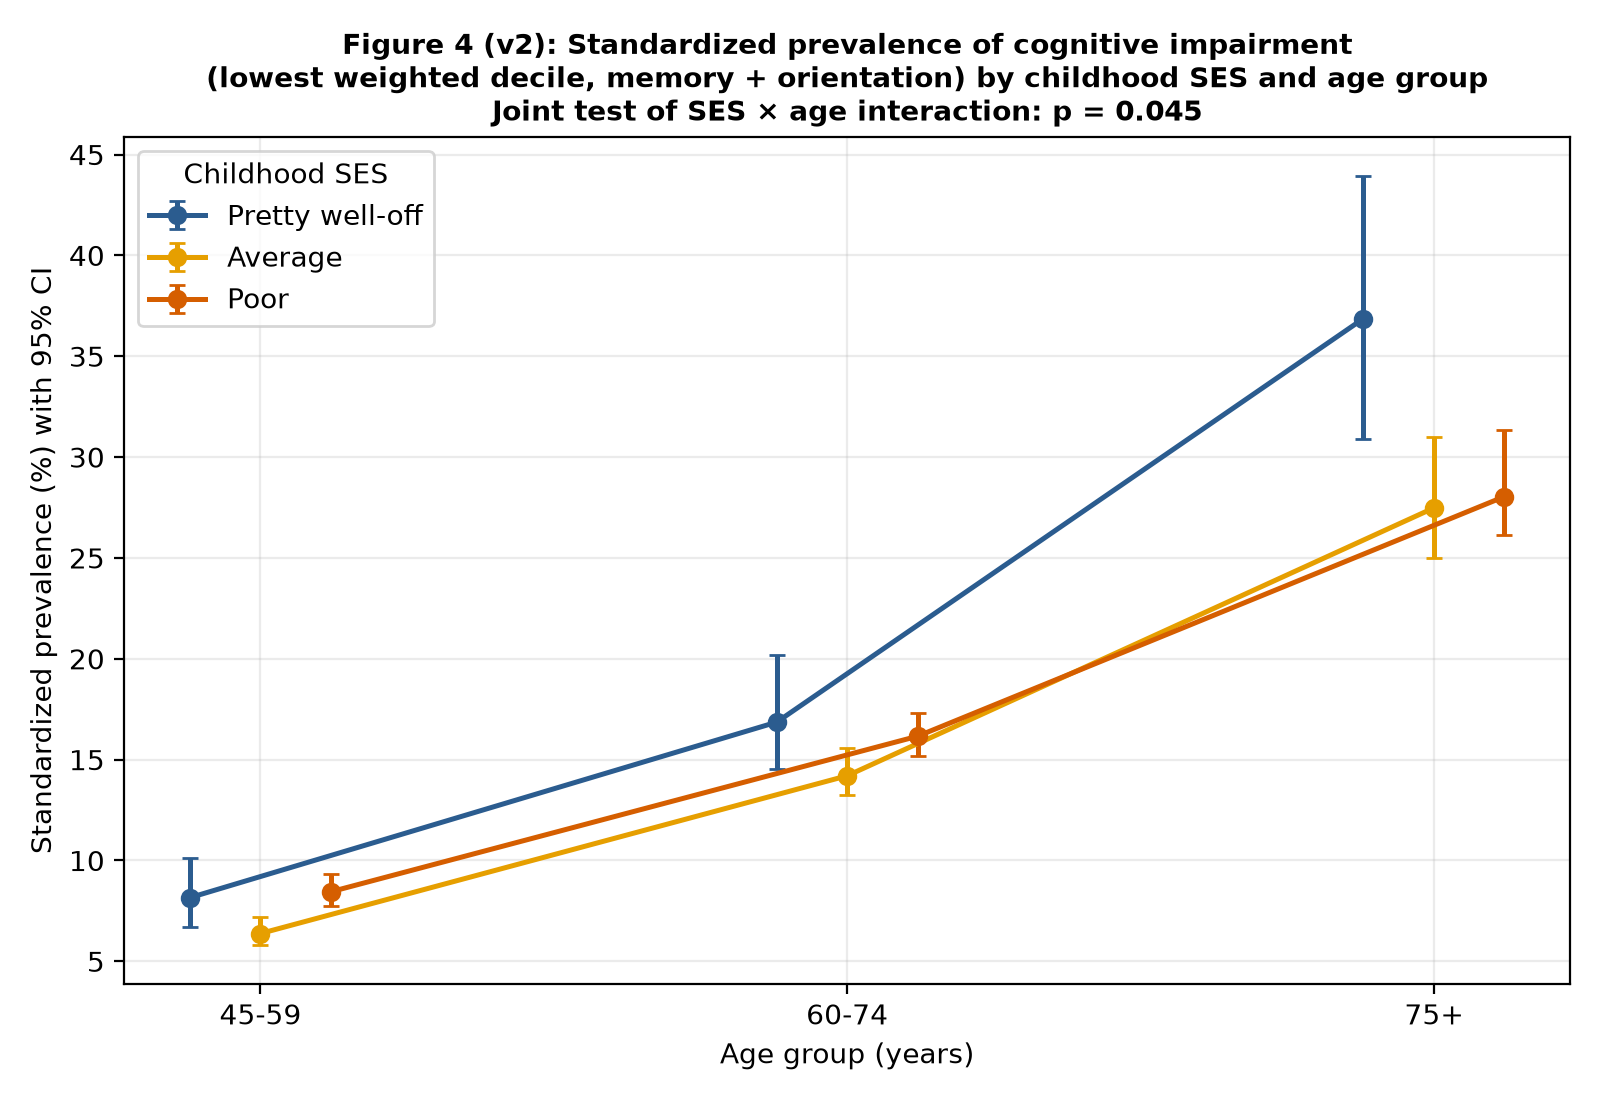
\includegraphics[width=\textwidth]{figures/figure4v2_cognition_interaction.png}
        \caption{Cognitive Impairment by Age}
        \label{fig:cog_inter}
    \end{subfigure}
    \hfill
    \begin{subfigure}[b]{0.48\textwidth}
        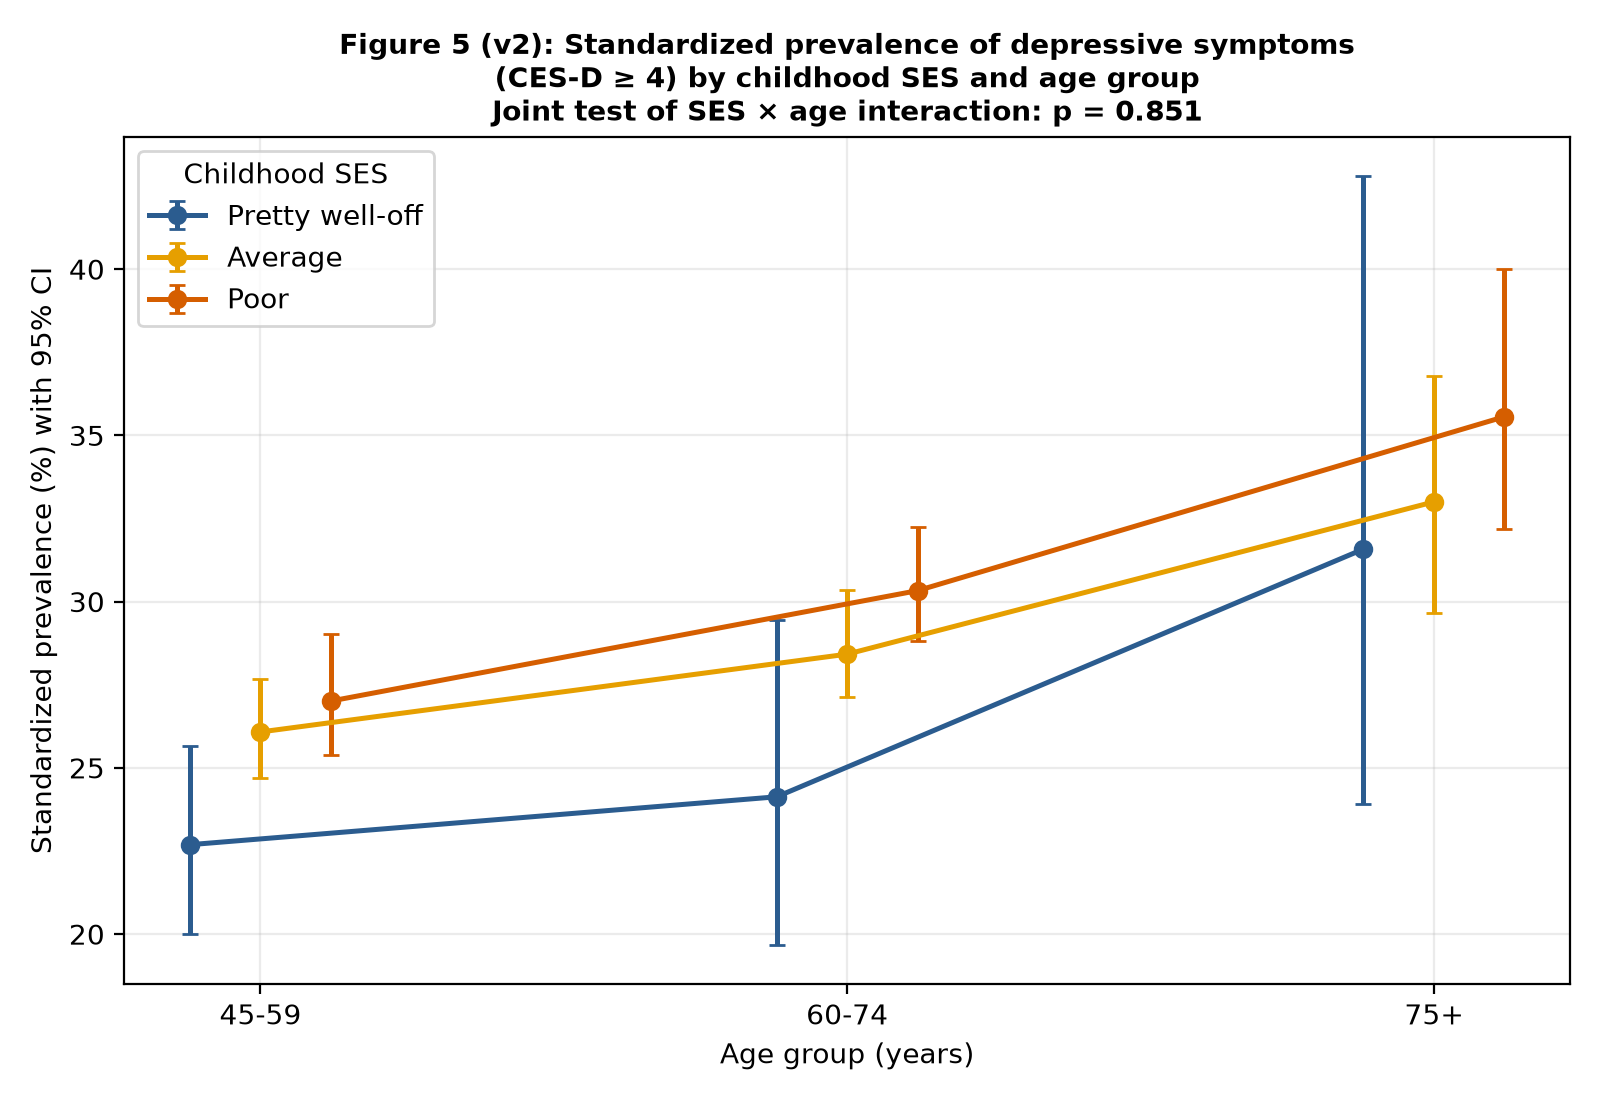
\includegraphics[width=\textwidth]{figures/figure5v2_depression_interaction.png}
        \caption{Depressive Symptoms by Age}
        \label{fig:dep_inter}
    \end{subfigure}
    \caption{\textbf{Adjusted Standardized Prevalences Across Age Groups by Childhood SES.} Average marginal predictions standardized over the empirical covariate distribution of each age group.}
    \label{fig:interactions}
\end{figure}

\section{Methodological Sensitivity and Robustness Analyses}

\subsection{Response Modeling and Inverse-Probability Weighting (IPW)}
To evaluate whether informative missingness in direct cognitive assessments introduced bias, we compared primary complete-case estimates against IPW-adjusted models (Table~\ref{tab:ipw}). The adjusted estimates for poor childhood SES ($\text{APR} = 0.928$ complete-case vs. $0.928$ IPW-adjusted) and poor childhood health ($\text{APR} = 0.949$ vs. $0.942$) were identical to the second decimal place, confirming that selection on measured covariates did not bias the primary conclusions.

\begin{table}[H]
\centering
\small
\caption{\textbf{Comparison of Complete-Case vs. IPW-Adjusted Model 2 Cognitive Estimates.}}
\label{tab:ipw}
\resizebox{0.85\textwidth}{!}{%
\begin{tabular}{lcc}
\toprule
\textbf{Childhood Exposure Parameter} & \textbf{Complete-Case APR (95\% CI)} & \textbf{IPW-Adjusted APR (95\% CI)} \\
\midrule
Childhood SES: Average & 0.797 (0.703--0.905) & 0.799 (0.708--0.903) \\
Childhood SES: Poor & 0.928 (0.818--1.052) & 0.928 (0.821--1.049) \\
Childhood health: Fair/Poor/Very poor & 0.949 (0.820--1.099) & 0.942 (0.811--1.094) \\
Childhood bedridden $\ge$1 month & 1.005 (0.860--1.176) & 1.003 (0.861--1.169) \\
\bottomrule
\end{tabular}%
}
\end{table}

\subsection{Measurement Sensitivity: The Cognitive Battery Conundrum}
A crucial finding emerged when comparing alternative cognitive outcome specifications:
\begin{itemize}
    \item \textbf{Memory and Orientation (Primary):} Poor childhood SES showed no association with impairment after adult education adjustment ($\text{APR} = 0.93$, 95\% CI: 0.82--1.05, $p = 0.241$). Stratifying by schooling confirmed that childhood poverty was not associated with impairment among unschooled adults ($\text{APR} = 0.91$, 95\% CI: 0.79--1.05) or schooled adults ($\text{APR} = 0.99$, 95\% CI: 0.76--1.29).
    \item \textbf{Skip-Aware Full Battery (\% of max):} When numeracy, executive function, and naming tasks were included, poor childhood SES remained significantly associated with impairment ($\text{APR} = 1.29$, 95\% CI: 1.07--1.57, $p = 0.009$), as did poor childhood health ($\text{APR} = 1.22$, 95\% CI: 1.08--1.37, $p = 0.001$).
\end{itemize}
This critical discrepancy demonstrates that conclusions regarding cognitive attenuation in LMICs depend entirely on the cognitive domains included. Tasks requiring formal manipulation of symbols (arithmetic, serial 7s) may retain residual educational confounding that standard categorical schooling adjustments cannot fully eradicate.

\subsection{Additional Robustness Checks}
Further sensitivity checks confirmed the integrity of our primary models:
\begin{itemize}
    \item \textbf{Modified Poisson vs. Logistic Regression:} For depression, the logistic odds ratio ($\text{AOR} = 1.33$, 95\% CI: 1.12--1.58) substantially overstated the effect relative to modified Poisson ($\text{APR} = 1.20$, 95\% CI: 1.07--1.34), confirming the methodological necessity of modified Poisson regression for common outcomes.
    \item \textbf{Continuous CES-D Scale:} Poor childhood health was associated with a $+0.37$ point elevation in continuous CES-D score ($p < 0.001$), and poor childhood SES with a $+0.32$ point elevation ($p < 0.001$).
    \item \textbf{Extreme Age Truncation:} Excluding adults aged $\ge 100$ ($N = 58$) yielded identical findings for depression ($\text{APR} = 1.20$) and cognition ($\text{APR} = 0.93$).
    \item \textbf{Varied SES Category:} Retaining the voluntary ``Varied'' SES category ($N = 421$) did not alter the main effect estimates.
\end{itemize}

\section{Discussion and Policy Implications}

\subsection{Substantive Divergence: Psychological Scarring vs. Cognitive Plasticity}
Our findings reveal a profound empirical divergence between mental and cognitive health in late life:
\begin{enumerate}
    \item \textbf{Enduring Somatic Scarring on Mental Health:} Early-life physical illness and economic adversity exert persistent associations with later-life depressive symptoms that remain evident 50 to 70 years after the exposure. Crucially, these associations cannot be accounted for by adult socioeconomic mobility, chronic physical disease, or current subjective health ratings. Early systemic inflammation, prolonged stress activation, or internalized experiences of childhood precarity appear to establish a persistent psychological vulnerability across the life span.
    \item \textbf{Cognitive Attenuation and the Education Nexus:} In contrast, early socioeconomic associations with memory and orientation are largely eliminated once adult schooling and consumption expenditure are accounted for. Formal schooling appears to confer cognitive reserve or functional scaffolding that protects against memory impairment, even among adults who grew up in extreme poverty.
\end{enumerate}

\subsection{Evaluation of Pre-Specified Hypotheses}
Table~\ref{tab:hypo_summary} summarizes the empirical verdicts for all five pre-specified hypotheses.

\begin{table}[H]
\centering
\small
\caption{\textbf{Empirical Verdicts for Pre-Specified Study Hypotheses.}}
\label{tab:hypo_summary}
\begin{tabularx}{\textwidth}{lXX}
\toprule
\textbf{Hypothesis} & \textbf{Cognitive Impairment Verdict} & \textbf{Depressive Symptoms Verdict} \\
\midrule
\textbf{H1: Childhood SES} & Supported in demographic models ($\text{APR}=1.36$), fully attenuated by adult SES ($\text{APR}=0.93$). & \textbf{Supported}: Persistent association in Model 2 ($\text{APR}=1.21$, 95\% CI: 1.03--1.42). \\
\addlinespace
\textbf{H2: Childhood Health} & \textbf{Not supported} on memory ($\text{APR}=0.95$), but supported on full battery ($\text{APR}=1.22$). & \textbf{Supported}: Persistent across all models ($\text{APR}=1.20$, 95\% CI: 1.07--1.34). \\
\addlinespace
\textbf{H3: Bedridden Illness} & \textbf{Not supported} ($\text{APR}=1.00$, 95\% CI: 0.86--1.18). & \textbf{Supported}: Persistent association ($\text{APR}=1.16$, 95\% CI: 1.05--1.28). \\
\addlinespace
\textbf{H4: Age Heterogeneity} & \textbf{Not supported}: One nominal test ($p=0.045$) in opposite direction in oldest-old. & \textbf{Not supported}: Uniform across age groups (all joint $p > 0.70$). \\
\addlinespace
\textbf{H5: Adult Attenuation} & Strong attenuation for childhood SES; caution against over-interpreting as causal mediation. & Partial attenuation for SES ($\approx 30\%$); minimal attenuation for childhood health. \\
\bottomrule
\end{tabularx}
\end{table}

\subsection{Strengths and Limitations}
\subsubsection{Methodological Strengths}
\begin{itemize}
    \item \textbf{Rigorous Survey Design Modeling:} Incorporation of 72 strata, 2,428 clusters, and 2,356 degrees of freedom using Taylor series linearization.
    \item \textbf{Modified Poisson Estimation:} Avoidance of odds-ratio inflation for common outcomes.
    \item \textbf{Measurement-Fair Cognitive Battery:} Resolution of literacy-skip scoring artifacts through a standardized memory and orientation composite.
    \item \textbf{Common Complete-Case Samples:} Prevention of artificial model-to-model sample fluctuations.
    \item \textbf{Transparent Post-Audit Protocol Amendment:} Complete documentation of initial analytical limitations and post-audit corrections.
\end{itemize}

\subsubsection{Study Limitations}
\begin{itemize}
    \item \textbf{Cross-Sectional Baseline:} LASI Wave 1 cannot establish individual longitudinal trajectories, disease incidence, or causal mediation over time.
    \item \textbf{Retrospective Recall Bias:} Childhood conditions were recalled at older ages, creating potential for mood-congruent recall error among currently depressed individuals.
    \item \textbf{Mortality / Survivor Selection:} Disadvantaged cohorts in LMICs experienced high childhood and mid-life mortality regimes, potentially biasing observed late-life associations toward the null.
    \item \textbf{Cognitive Non-Response:} Proxy interviews ($N = 705$) were excluded from cognitive testing, omitting the most severely impaired older adults.
\end{itemize}

\subsection{Public Health and Policy Implications}
Current ageing policies in India, including the National Programme for the Health Care of the Elderly (NPHCE), focus predominantly on late-life tertiary geriatric care and chronic disease management. While vital, our findings demonstrate that healthy cognitive and mental ageing begins decades before adulthood. Preventing late-life depression requires upstream investments in maternal-child health, childhood disease prevention, and family economic security. Simultaneously, expanding universal secondary and higher education provides the most robust institutional pathway for building long-term cognitive resilience in developing nations.

\section{Conclusions with Empirical Evidence}
\begin{enumerate}
    \item \textbf{Persistent Mental Health Disparities:} Poor childhood health ($\text{APR} = 1.20$, 95\% CI: 1.07--1.34, $p = 0.002$), poor childhood SES ($\text{APR} = 1.21$, 95\% CI: 1.03--1.42, $p = 0.019$), and childhood bedridden illness ($\text{APR} = 1.16$, 95\% CI: 1.05--1.28, $p = 0.005$) are independently associated with elevated depressive symptoms in late life. Each additional adversity confers an 11.4\% elevation in depressive symptoms ($\text{APR} = 1.114$, $p < 0.001$).
    \item \textbf{Education-Dependent Cognitive Trajectories:} In memory and orientation assessments, the childhood poverty penalty ($\text{APR} = 1.36$ in demographic models) is fully attenuated by adult education and consumption expenditure ($\text{APR} = 0.93$, 95\% CI: 0.82--1.05). However, residual disparities persist on complex numeracy tasks, highlighting the critical sensitivity of cognitive findings to battery design.
    \item \textbf{Uniformity Across Age Strata:} Formal joint interaction tests confirm that early disadvantage associations do not widen across ageing cohorts, demonstrating stable lifelong disparities rather than cumulative divergence.
    \item \textbf{Empirical Bottom Line:} Maternal and child health investments and equitable access to schooling represent foundational public health strategies for ensuring cognitive and mental vitality in an ageing India.
\end{enumerate}

\section*{Reproducibility and Data Availability}
All analytic scripts are preserved in the project repository:
\begin{itemize}
    \item Dataset extraction and standardization: \texttt{code/07\_build\_dataset\_v2.py}
    \item Design-based survey inference engine: \texttt{code/survey\_utils.py}
    \item Core regression and interaction modeling: \texttt{code/08\_models\_v2.py}
    \item Forest plot visualization: \texttt{code/09\_forest\_plot\_v2.py}
    \item HTML report generator: \texttt{code/10\_generate\_report\_v2.py}
    \item LaTeX report generator: \texttt{code/11\_generate\_latex_report.py}
\end{itemize}

\end{document}
